\documentclass[10]{article}
%\documentclass[11pt]{book}
\usepackage{hyperref}
\usepackage{amsfonts,amssymb,amsmath,amsthm,cite}
%\usepackage{graphicx}
\usepackage[toc,page]{appendix}
\usepackage{nicefrac}
%% \usepackage[francais]{babel}
\usepackage[applemac]{inputenc}
\usepackage{amssymb, euscript}
\usepackage[matrix,arrow,curve]{xy}
\usepackage{graphicx}
\usepackage{tabularx}
\usepackage{float}
\usepackage{tikz}
\usepackage{slashed}
\usepackage{mathrsfs}
\usepackage{multirow}
\usepackage{rotating}

%\usepackage{mathtools}

\usetikzlibrary{matrix}
\usetikzlibrary{cd}

\usepackage{siunitx}

\usepackage{lmodern}
\usepackage[T1]{fontenc}
\usepackage[babel=true]{microtype}


\usepackage{amsfonts,cite}
\usepackage{graphicx}

%% \usepackage[francais]{babel}
\usepackage[applemac]{inputenc}


\usepackage[sc]{mathpazo}
\usepackage{environ}

\linespread{1.05}         % Palatino needs more leading (space between lines)


%\usepackage[usenames]{color}



\DeclareFontFamily{T1}{pzc}{}
\DeclareFontShape{T1}{pzc}{m}{it}{1.8 <-> pzcmi8t}{}
\DeclareMathAlphabet{\mathpzc}{T1}{pzc}{m}{it}
\DeclareMathOperator{\cosupp}{\mathfrak{cosupp}}            %% 
% the command for it is \mathpzc

\textwidth=140mm


% % % % % % % % % % % % % % % % % % % %
\theoremstyle{plain}
\newtheorem{prop}{Proposition}[section]
\newtheorem{prdf}[prop]{Proposition and Definition}
\newtheorem{lem}[prop]{Lemma}%[section]
\newtheorem{cor}[prop]{Corollary}%[section]
\newtheorem{thm}[prop]{Theorem}%[section]
\newtheorem{theorem}[prop]{Theorem}
\newtheorem{lemma}[prop]{Lemma}
\newtheorem{proposition}[prop]{Proposition}
\newtheorem{corollary}[prop]{Corollary}
\newtheorem{statement}[prop]{Statement}

\theoremstyle{definition}
\newtheorem{defn}[prop]{Definition}%[section]
\newtheorem{cordefn}[prop]{Corollary and Definition}%[section]
\newtheorem{empt}[prop]{}%[section]
\newtheorem{exm}[prop]{Example}%[section]
\newtheorem{rem}[prop]{Remark}%[section]
\newtheorem{prob}[prop]{Problem}
\newtheorem{conj}{Conjecture}       %% Hypothesis 1
\newtheorem{cond}{Condition}        %% Condition 1
%\newtheorem{axiom}[thm]{Axiom}           %% Axiom 1 modified
\newtheorem{fact}[prop]{Fact}
\newtheorem{ques}{Question}         %% Question 1
\newtheorem{answ}{Answer}           %% Answer 1
\newtheorem{notn}{Notation}        %% Notations are not numbered

\theoremstyle{definition}
\newtheorem{notation}[prop]{Notation}
\newtheorem{definition}[prop]{Definition}
\newtheorem{example}[prop]{Example}
\newtheorem{exercise}[prop]{Exercise}
\newtheorem{conclusion}[prop]{Conclusion}
\newtheorem{conjecture}[prop]{Conjecture}
\newtheorem{criterion}[prop]{Criterion}
\newtheorem{summary}[prop]{Summary}
\newtheorem{axiom}[prop]{Axiom}
\newtheorem{problem}[prop]{Problem}
%\theoremstyle{remark}
\newtheorem{remark}[prop]{Remark}

\numberwithin{equation}{section}
\newtheorem*{claim}{Claim}
\DeclareMathOperator{\Dom}{Dom}              %% domain of an operator
\newcommand{\Dslash}{{D\mkern-11.5mu/\,}}    %% Dirac operator
\newcommand{\trG}{{\rm tr}_G\;}
\newcommand{\trF}{{\rm tr}_{\cal F}\;}
\newcommand{\TR}{{\rm TR}\;}
\newcommand{\res}{{\rm res}\;}


\newcommand\ci{${\mathcal C}^{\infty}$}
\newcommand\CI{{\mathcal C}^{\infty}}
\newcommand\CIc{{\mathcal C}^{\infty}_{\text{c}}}

%\newcommand\myeq{\stackrel{\mathclap{\normalfont\mbox{def}}}{=}}
\newcommand{\rar}[1]{\stackrel{#1}{\longrightarrow}}
\newcommand{\lar}[1]{\stackrel{#1}{\longleftarrow}}

\newcommand{\nor}[1]{\left\Vert #1\right\Vert}    %\nor{x}=||x||
\newcommand{\norm}[1]{\left\| #1\right\|}    %\nor{x}=||x||
\newcommand{\vertiii}[1]{{\left\vert\kern-0.25ex\left\vert\kern-0.25ex\left\vert #1
		\right\vert\kern-0.25ex\right\vert\kern-0.25ex\right\vert}}
\newcommand{\Ga}{\Gamma}  
\newcommand{\coker}{\mathrm{coker}}                   %% short for  \Gamma
\newcommand{\Coo}{C^\infty}                  %% smooth functions
\newcommand{\dom}{\mathrm{dom}}                  %% smooth functions
\newcommand{\Cont}{C} 
\newcommand{\cl}{\overline} 
\newcommand{\Contc}{C_c} 
\newcommand{\Contb}{C_b} 
\newcommand{\Repi}{\mathrm{Rep}_{int}} 
\newcommand{\Rep}{\mathrm{Rep}} 
\newcommand{\hor}[0]{\mathrm{hor}}
\newcommand{\comp}{\operatorname{comp}}
\newcommand{\adb}{\operatorname{adb}}
\newcommand{\dist}{\operatorname{dist}}


% % % % % % % % % % % % % % % % % % % %


\usepackage[sc]{mathpazo}
\linespread{1.05}         % Palatino needs more leading (space between lines)

\newbox\ncintdbox \newbox\ncinttbox %% noncommutative integral symbols
\setbox0=\hbox{$-$} \setbox2=\hbox{$\displaystyle\int$}
\setbox\ncintdbox=\hbox{\rlap{\hbox
		to \wd2{\hskip-.125em \box2\relax\hfil}}\box0\kern.1em}
\setbox0=\hbox{$\vcenter{\hrule width 4pt}$}
\setbox2=\hbox{$\textstyle\int$} \setbox\ncinttbox=\hbox{\rlap{\hbox
		to \wd2{\hskip-.175em \box2\relax\hfil}}\box0\kern.1em}

\newcommand{\ncint}{\mathop{\mathchoice{\copy\ncintdbox}%
		{\copy\ncinttbox}{\copy\ncinttbox}%
		{\copy\ncinttbox}}\nolimits}  %% NC integral

%%% Repeated relations:
\newcommand{\xyx}{\times\cdots\times}      %% repeated product
\newcommand{\opyop}{\oplus\cdots\oplus}    %% repeated direct sum
\newcommand{\oxyox}{\otimes\cdots\otimes}  %% repeated tensor product
\newcommand{\wyw}{\wedge\cdots\wedge}      %% repeated exterior product
\newcommand{\subysub}{\subset\hdots\subset}      %% repeated subset
\newcommand{\supysup}{\supset\hdots\supset}      %% repeated supset
\newcommand\CC{\mathbb C}
\newcommand\NN{\mathbb N}
\newcommand\RR{\mathbb R}
\newcommand\ZZ{\mathbb Z}
\newcommand{\LGR}{\matcal L}
\newcommand{\rep}{\mathfrak{rep}}
\newcommand{\lift}{\mathfrak{lift}}
\newcommand{\desc}{\mathfrak{desc}}
\newcommand{\Cstar}{C^*}
\newcommand{\Cst}{C^*}
\newcommand{\Star}{*}
\newcommand{\PS}[1]{\Psi^{#1}(\GR;E)}

%%% Roman letters:
\newcommand{\id}{\mathrm{id}}                %% identity map
\newcommand{\Id}{\mathrm{Id}}                %% identity map
\newcommand{\pt}{\mathrm{pt ???}}                %% a point
\newcommand{\const}{\mathrm{const}}          %% a constant
\newcommand{\codim}{\mathrm{codim}}          %% codimension
\newcommand{\cyc}{\mathrm{cyclic}}  %% cyclic sum
\renewcommand{\d}{\mathrm{d}}       %% commutative differential
\newcommand{\dR}{\mathrm{dR}}       %% de~Rham cohomology
\newcommand{\proj}{\mathrm{proj}}                %% a projection
\newcommand*{\braket}[2]{\langle#1 {,~} #2\rangle}% right inner products
\newcommand*{\lbraket}[2]{\langle\!\langle#1{\mid}#2\rangle\!\rangle}% left inner products

\newcommand*{\Mult}{\mathcal M}% multiplier algebra
\newcommand{\Lt}{\mathcal{L}}                 %%\newcommand{\unitsv}[1]{#1^{(0)}}

\newcommand{\A}{\mathcal{A}}                 %%\newcommand{\unitsv}[1]{#1^{(0)}}
\newcommand{\units}{G^{(0)}}
\newcommand{\haars}{\{\lambda^{u}\}_{u\in\units}}
\newcommand{\shaars}{\{\lambda_{u}\}_{u\in\units}}
\newcommand{\haarsv}[2]{\{\lambda^{#2}_{#1}\}_{#2\in\unitsv{#1}}}
\newcommand{\haarv}[2]{\lambda^{#2}_{#1}}

\renewcommand{\a}{\alpha}                    %% short for  \alphapha
\DeclareMathOperator{\ad}{ad}                %% infml adjoint repn
\newcommand{\as}{\quad\mbox{as}\enspace}     %% `as' with spacing
\newcommand{\Aun}{\widetilde{\mathcal{A}}}   %% unital algebra
\newcommand{\B}{\mathcal{B}}                 %% space of distributions
\newcommand{\E}{\mathcal{E}}                 %% space of distributions
\renewcommand{\b}{\beta}                     %% short for \beta
\newcommand{\braCket}[3]{\langle#1\mathbin|#2\mathbin|#3\rangle}
%\newcommand{\braket}[2]{\langle#1\mathbin|#2\rangle} %% <w|z>
\newcommand{\C}{\mathbb{C}}                  %% complex numbers
\newcommand{\cc}{\mathbf{c}}                 %% Hochschild cycle
\DeclareMathOperator{\Cl}{C\ell}             %% Clifford algebra
\newcommand{\F}{\mathcal{F}}                 %% space of test functions
\newcommand{\G}{\mathcal{G}}                 %% 
\newcommand{\GR}{\mathcal{G}}                 %% 
\newcommand{\D}{\mathcal{D}}                 %% Moyal L^2-filtration
\renewcommand{\H}{\mathcal{H}}               %% Hilbert space
\newcommand{\half}{\tfrac{1}{2}}             %% small fraction  1/2
\newcommand{\hh}{\mathcal{H}}                %% Hilbert space
\newcommand{\hookto}{\hookrightarrow}        %% abbreviation
\newcommand{\Ht}{{\widetilde{\mathcal{H}}}}  %% Hilbert space of forms
\newcommand{\I}{\mathcal{I}}                 %% tracelike functions
\DeclareMathOperator{\Junk}{Junk}            %% the junk DGA ideal
\newcommand{\K}{\mathcal{K}}                 %% compact operators
\newcommand{\ket}[1]{|#1\rangle}             %% ket vector
\newcommand{\ketbra}[2]{|#1\rangle\langle#2|} %% rank one operator
\renewcommand{\L}{\mathcal{L}}               %% operator algebra
\newcommand{\La}{\Lambda}                    %% short for \Lambda
\newcommand{\la}{\lambda}                    %% short for \lambda
\newcommand{\lf}{L_f^\theta}                 %% left  mult operator
\newcommand{\M}{\mathcal{M}}                 %% Moyal multplr algebra
\newcommand{\Lb}{\mathcal{L}}                 %% Moyal multplr algebra
\newcommand{\mm}{\mathcal{M}^\theta}
%\newcommand{{{\star_{\theta}}}{{\mathchoice{\mathbin{\;|\;ar_{_\theta}}}
			%            {\mathbin{\;|\;ar_{_\theta}}}           %% Moyal
			%            {{\;|\;ar_\theta}}{{\;|\;ar_\theta}}}}    %% product
	\newcommand{\N}{\mathbb{N}}                  %%  integers
	\newcommand{\nb}{\nabla}                     %% gradient
	\newcommand{\Oh}{\mathcal{O}}                %% comm multiplier alg
	\newcommand{\om}{\omega}                     %% short for \omega
	\newcommand{\opp}{{\mathrm{op}}}             %% opposite algebra
	\newcommand{\ox}{\otimes}                    %% tensor product
	\newcommand{\eps}{\varepsilon}                    %% tensor product
	\newcommand{\otimesyox}{\otimes\cdots\otimes}    %% repeated tensor product
	\newcommand{\pa}{\partial}                   %% short for \partial
	\newcommand{\pd}[2]{\frac{\partial#1}{\partial#2}}%% partial derivative
	\newcommand{\piso}[1]{\lfloor#1\rfloor}      %% integer part
	\newcommand{\PsiDO}{\Psi~\mathrm{DO}}         %% pseudodiffl operators
	\newcommand{\Q}{\mathbb{Q}}                  %% rational numbers
	\newcommand{\R}{\mathbb{R}}                  %% real numbers
	\newcommand{\rdl}{R_\Dslash(\lambda)}        %% resolvent
	\newcommand{\roundbraket}[2]{(#1\mathbin|#2)} %% (w|z)
	\newcommand{\row}[3]{{#1}_{#2},\dots,{#1}_{#3}} %% list: a_1,...,a_n
	\newcommand{\sepword}[1]{\quad\mbox{#1}\quad} %% well-spaced words
	\newcommand{\set}[1]{\{\,#1\,\}}             %% set notation
	\newcommand{\Sf}{\mathbb{S}}                 %% sphere
	\newcommand{\uhor}[1]{\Omega^1_{hor}#1}
	\newcommand{\sco}[1]{{\sp{(#1)}}}
	\newcommand{\sw}[1]{{\sb{(#1)}}}
	\DeclareMathOperator{\spec}{sp}              %% spectrum
	\renewcommand{\SS}{\mathcal{S}}              %% Schwartz space
	\newcommand{\sss}{\mathcal{S}}               %% Schwartz space
	\DeclareMathOperator{\supp}{\mathfrak{supp}}            %% support
	\newcommand{\T}{\mathbb{T}}                  %% circle as a group
	\renewcommand{\th}{\theta}                   %% short for \theta
	\newcommand{\thalf}{\tfrac{1}{2}}            %% small* fraction 1/2
	\newcommand{\tihalf}{\tfrac{i}{2}}           %% small* fraction i/2
	\newcommand{\tpi}{{\tilde\pi}}               %% extended representation
	\DeclareMathOperator{\Tr}{Tr}                %% trace of operator
	\DeclareMathOperator{\tr}{tr}                %% trace of matrix
	\newcommand{\del}{\partial}                  %% short for  \partial
	\DeclareMathOperator{\tsum}{{\textstyle\sum}} %% small sum in display
	\newcommand{\V}{\mathcal{V}}                 %% test function space
	\newcommand{\vac}{\ket{0}}                   %% vacuum ket vector
	\newcommand{\vf}{\varphi}                    %% scalar field
	\newcommand{\w}{\wedge}                      %% exterior product
	\DeclareMathOperator{\wres}{wres}            %% density of Wresidue
	\newcommand{\x}{\times}                      %% cross
	\newcommand{\Z}{\mathbb{Z}}                  %% integers
	\newcommand{\7}{\dagger}                     %% short for + symbol
	\newcommand{\8}{\bullet}                     %% anonymous degree
	\renewcommand{\.}{\cdot}                     %% anonymous variable
	\renewcommand{\:}{\colon}                    %% colon in  f: A -> B
	
	%\newcommand{\sA}{\mathscr{A}}       %%
	\newcommand{\sA}{\mathcal{A}} 
	\newcommand{\sB}{\mathcal{B}}       %%
	\newcommand{\sC}{\mathcal{C}}       %%
	\newcommand{\sD}{\mathcal{D}}       %%
	\newcommand{\sE}{\mathcal{E}}       %%
	\newcommand{\sF}{\mathcal{F}}       %%
	\newcommand{\sG}{\mathcal{G}}       %%
	\newcommand{\sH}{\mathcal{H}}       %%
	\newcommand{\sI}{\mathcal{I}}       %%
	\newcommand{\sJ}{\mathcal{J}}       %%
	\newcommand{\sK}{\mathcal{K}}       %%
	\newcommand{\sL}{\mathcal{L}}       %%
	\newcommand{\sM}{\mathcal{M}}       %%
	\newcommand{\sN}{\mathcal{N}}       %%
	\newcommand{\sO}{\mathcal{O}}       %%
	\newcommand{\sP}{\mathcal{P}}       %%
	\newcommand{\sQ}{\mathcal{Q}}       %%
	\newcommand{\sR}{\mathcal{R}}       %%
	\newcommand{\sS}{\mathcal{S}}       %%
	\newcommand{\sT}{\mathcal{T}}       %%
	\newcommand{\sU}{\mathcal{U}}       %%
	\newcommand{\sV}{\mathcal{V}}       %%
	\newcommand{\sX}{\mathcal{X}}       %%
	\newcommand{\sY}{\mathcal{Y}}       %%
	\newcommand{\sZ}{\mathcal{Z}}       %%
	
	\newcommand{\Om}{\Omega}       %%
	
	
	\DeclareMathOperator{\ptr}{ptr}     %% Poisson trace
	\DeclareMathOperator{\Trw}{Tr_\omega} %% Dixmier trace
	\DeclareMathOperator{\vol}{Vol}     %% total volume
	\DeclareMathOperator{\Vol}{Vol}     %% total volume
	\DeclareMathOperator{\Area}{Area}   %% area of a surface
	\DeclareMathOperator{\Wres}{Wres}   %% (Wodzicki) residue
	
	\newcommand{\dd}[1]{\frac{\partial}{\partial#1}}   %% partial derivation
	\newcommand{\ddt}[1]{\frac{d}{d#1}}                %% derivative
	\newcommand{\inv}[1]{\frac{1}{#1}}                 %% inverse
	\newcommand{\sfrac}[2]{{\scriptstyle\frac{#1}{#2}}} %% tiny fraction
	
	\newcommand\VD{{\mathcal D}}
	\newcommand{\bA}{\mathbb{A}}       %%
	\newcommand{\bB}{\mathbb{B}}       %%
	\newcommand{\bC}{\mathbb{C}}       %%
	\newcommand{\bCP}{\mathbb{C}P}     %%
	\newcommand{\bD}{\mathbb{D}}       %%
	\newcommand{\bE}{\mathbb{E}}       %%
	\newcommand{\bF}{\mathbb{F}}       %%
	\newcommand{\bG}{\mathbb{G}}       %%
	\newcommand{\bH}{\mathbb{H}}       %%
	\newcommand{\bHP}{\mathbb{H}P}     %%
	\newcommand{\bI}{\mathbb{I}}       %%
	\newcommand{\bJ}{\mathbb{J}}       %%
	\newcommand{\bK}{\mathbb{K}}       %%
	\newcommand{\bL}{\mathbb{L}}       %%
	\newcommand{\bM}{\mathbb{M}}       %%
	\newcommand{\bN}{\mathbb{N}}       %%
	\newcommand{\bO}{\mathbb{O}}       %%
	\newcommand{\bOP}{\mathbb{O}P}     %%
	\newcommand{\bP}{\mathbb{P}}       %%
	\newcommand{\bQ}{\mathbb{Q}}       %%
	\newcommand{\bR}{\mathbb{R}}       %%
	\newcommand{\bRP}{\mathbb{R}P}     %%
	\newcommand{\bS}{\mathbb{S}}       %%
	\newcommand{\bT}{\mathbb{T}}       %%
	\newcommand{\bU}{\mathbb{U}}       %%
	\newcommand{\bV}{\mathbb{V}}       %%
	\newcommand{\bX}{\mathbb{X}}       %%
	\newcommand{\bY}{\mathbb{Y}}       %%
	\newcommand{\bZ}{\mathbb{Z}}       %%
	
	\newcommand{\bydef}{\stackrel{\mathrm{def}}{=}}          %% 
	\newcommand{\defeq}{\stackrel{\mathrm{def}}{=}}   
	
	
	
	\newcommand{\al}{\alpha}          %% short for  \alpha
	\newcommand{\bt}{\beta}           %% short for  \beta
	\newcommand{\Dl}{\Delta}          %% short for  \Delta
	\newcommand{\dl}{\delta}          %% short for  \delta
	\newcommand{\ga}{\gamma}          %% short for  \gamma
	\newcommand{\ka}{\kappa}          %% short for  \kappa
	\newcommand{\sg}{\sigma}          %% short for  \sigma
	\newcommand{\Sg}{\Sigma}          %% short for  \Sigma
	\newcommand{\Th}{\Theta}          %% short for  \Theta
	\renewcommand{\th}{\theta}        %% short for  \theta
	\newcommand{\vth}{\vartheta}      %% short for  \vartheta
	\newcommand{\ze}{\zeta}           %% short for  \zeta
	
	\DeclareMathOperator{\ord}{ord}     %% order of a PsiDO
	\DeclareMathOperator{\rank}{rank}   %% rank of a vector bundle
	\DeclareMathOperator{\sign}{sign}   %%
	\DeclareMathOperator{\sgn}{sgn}   %%
	\DeclareMathOperator{\chr}{char}   %%
	\DeclareMathOperator{\ev}{ev}       %% evaluation
	
	\newcommand{\Op}{\mathbf{Op}}
	\newcommand{\As}{\mathbf{As}}
	\newcommand{\Com}{\mathbf{Com}}
	\newcommand{\LLie}{\mathbf{Lie}}
	\newcommand{\Leib}{\mathbf{Leib}}
	\newcommand{\Zinb}{\mathbf{Zinb}}
	\newcommand{\Poiss}{\mathbf{Poiss}}
	
	\newcommand{\gX}{\mathfrak{X}}      %% vector fields
	\newcommand{\sol}{\mathfrak{so}}    %% special orthogonal Lie algebra
	\newcommand{\gm}{\mathfrak{m}}      %% maximal ideal
	
	
	\DeclareMathOperator{\Res}{Res}
	\DeclareMathOperator{\NCRes}{NCRes}
	\DeclareMathOperator{\Ind}{Ind}
	%% co/homology theories
	\DeclareMathOperator{\rH}{H}        %% any co/homology
	\DeclareMathOperator{\rC}{C}        %%  any co/chains
	\DeclareMathOperator{\rZ}{Z}        %% cycles
	\DeclareMathOperator{\rB}{B}        %% boundaries
	\DeclareMathOperator{\rF}{F}        %% filtration
	\DeclareMathOperator{\Gr}{gr}        %% associated graded object
	\DeclareMathOperator{\rHc}{H_{\mathrm{c}}}   %% co/homology with compact support
	\DeclareMathOperator{\drH}{H_{\mathrm{dR}}}  %% de Rham co/homology
	\DeclareMathOperator{\cechH}{\check{H}}    %% Cech co/homology
	\DeclareMathOperator{\rK}{K}        %% K-groups
	\DeclareMathOperator{\rKO}{KO}        %% real K-groups
	\DeclareMathOperator{\rKU}{KU}        %% unitary K-groups
	\DeclareMathOperator{\rKSp}{KSp}        %% symplectic K-groups
	\DeclareMathOperator{\rR}{R}        %% representation ring
	\DeclareMathOperator{\rI}{I}        %% augmentation ideal
	\DeclareMathOperator{\HH}{HH}       %% Hochschild co/homology
	\DeclareMathOperator{\HC}{HC}       %% cyclic co/homology
	\DeclareMathOperator{\HP}{HP}       %% periodic cyclic co/homology
	\DeclareMathOperator{\HN}{HN}       %% negative cyclic co/homology
	\DeclareMathOperator{\HL}{HL}       %% Leibniz co/homology
	\DeclareMathOperator{\KK}{KK}       %% KK-theory
	\DeclareMathOperator{\KKK}{\mathbf{KK}}       %% KK-theory as a category
	\DeclareMathOperator{\Ell}{Ell}       %% Abstract elliptic operators
	\DeclareMathOperator{\cd}{cd}       %% cohomological dimension
	\DeclareMathOperator{\spn}{span}       %% span
	\DeclareMathOperator{\linspan}{span} %% linear span (can't use \span)
	\newcommand{\blank}{-}   
	
	
	
	\newcommand{\twobytwo}[4]{\begin{pmatrix} #1 & #2 \\ #3 & #4 \end{pmatrix}}
	\newcommand{\CGq}[6]{C_q\!\begin{pmatrix}#1&#2&#3\\#4&#5&#6\end{pmatrix}}
	%% q-Clebsch--Gordan coefficients
	\newcommand{\cz}{{\bullet}}         %% anonymous degree
	\newcommand{\nic}{{\vphantom{\dagger}}} %% invisible dagger
	\newcommand{\ep}{{\dagger}}         %% abbreviation for + symbol
	\newcommand{\downto}{\downarrow}    %% right hand limit
	\newcommand{\isom}{\cong}          %% isomorphism
	\newcommand{\lt}{\triangleright}    %% a left  action
	\newcommand{\otto}{\leftrightarrow} %% bijection
	\newcommand{\rt}{\triangleleft}     %% a right action
	\newcommand{\semi}{\rtimes}         %% crossed product
	\newcommand{\tensor}{\otimes}       %% tensor product
	\newcommand{\cotensor}{\square}       %% cotensor product
	\newcommand{\trans}{\pitchfork}     %% transverse
	\newcommand{\ul}{\underline}        %% for sheaves
	\newcommand{\upto}{\uparrow}        %% left  hand limit
	\renewcommand{\:}{\colon}           %% colon in  f: A -> B
	\newcommand{\blt}{\ast}
	\newcommand{\Co}{C_{\bullet}}
	\newcommand{\cCo}{C^{\bullet}}
	\newcommand{\nbs}{\nabla^S}         %% spin connection
	\newcommand{\up}{{\mathord{\uparrow}}} %% `up' spinors
	\newcommand{\dn}{{\mathord{\downarrow}}} %% `down' spinors
	\newcommand{\updn}{{\mathord{\updownarrow}}} %% up or down
	
	%%% Bilinear enclosures:
	
	\newcommand{\bbraket}[2]{\langle\!\langle#1\stroke#2\rangle\!\rangle}
	%% <<w|z>>
	\newcommand{\bracket}[2]{\langle#1,\, #2\rangle} %% <w,z>
	\newcommand{\scalar}[2]{\langle#1,\,#2\rangle} %% <w,z>
	\newcommand{\poiss}[2]{\{#1,\,#2\}} %% {w,z}
	\newcommand{\dst}[2]{\langle#1,#2\rangle} %% distributions <u,\phi>
	\newcommand{\pairing}[2]{(#1\stroke #2)} %% right-linear pairing
	\def\<#1|#2>{\langle#1\stroke#2\rangle} %% \braket (Dirac notation)
	\def\?#1|#2?{\{#1\stroke#2\}}        %% left-linear pairing
	
	%%% Accent-like macros:
	
	\renewcommand{\Bar}[1]{\overline{#1}} %% closure operator
	\renewcommand{\Hat}[1]{\widehat{#1}}  %% short for \widehat
	\renewcommand{\Tilde}[1]{\widetilde{#1}} %% short for \widetilde
	
	
	\DeclareMathOperator{\bCl}{\bC l}   %% complex Clifford algebra
	
	%%% Small fractions in displays:
	
	\newcommand{\ihalf}{\tfrac{i}{2}}   %% small fraction  i/2
	\newcommand{\quarter}{\tfrac{1}{4}} %% small fraction  1/4
	\newcommand{\shalf}{{\scriptstyle\frac{1}{2}}}  %% tiny fraction  1/2
	\newcommand{\third}{\tfrac{1}{3}}   %% small fraction  1/3
	\newcommand{\ssesq}{{\scriptstyle\frac{3}{2}}} %% tiny fraction  3/2
	\newcommand{\sesq}{{\mathchoice{\tsesq}{\tsesq}{\ssesq}{\ssesq}}} %% 3/2
	\newcommand{\tsesq}{\tfrac{3}{2}}   %% small fraction  3/2
	
	
	%\newcommand\eqdef{\over set{\mathclap{\normalfont\mbox{def}}}{=}}
	\newcommand\eqdef{\over set{\mathrm{def}}{=}}
	
	
	%+++++++++++++++++++++++++++++++++++
	
	\newcommand{\word}[1]{\quad\text{#1}\enspace} %% well-spaced words
	\newcommand{\words}[1]{\quad\text{#1}\quad} %% better-spaced words
	\newcommand{\su}[1]{{\sp{[#1]}}}
	
	\def\<#1,#2>{\langle#1,#2\rangle}            %% bilinear pairing
	\def\ee_#1{e_{{\scriptscriptstyle#1}}}       %% basis projector
	\def\wick:#1:{\mathopen:#1\mathclose:}       %% Wick-ordered operator
	
	\newcommand{\opname}[1]{\mathop{\mathrm{#1}}\nolimits}
	
	\newcommand{\hideqed}{\renewcommand{\qed}{}} %% to suppress `\qed'
	
	
	%%%%%%%%%%%%%%%%%%%%%%%%%%%%%
	%% 2. Some internal machinery
	%%%%%%%%%%%%%%%%%%%%%%%%%%%%%
	
	\newbox\ncintdbox \newbox\ncinttbox %% noncommutative integral symbols
	\setbox0=\hbox{$-$}
	\setbox2=\hbox{$\displaystyle\int$}
	\setbox\ncintdbox=\hbox{\rlap{\hbox
			to \wd2{\box2\relax\hfil}}\box0\kern.1em}
	\setbox0=\hbox{$\vcenter{\hrule width 4pt}$}
	\setbox2=\hbox{$\textstyle\int$}
	\setbox\ncinttbox=\hbox{\rlap{\hbox
			to \wd2{\hskip-.05em\box2\relax\hfil}}\box0\kern.1em}
	
	\newcommand{\disp}{\displaystyle} %% short for  \displaystyle
	
	%\newcommand{\hideqed}{\renewcommand{\qed}{}} %% no `\qed' at end-proof
	
	\newcommand{\stroke}{\mathbin|}   %% (for `\bbraket' and such)
	\newcommand{\tribar}{|\mkern-2mu|\mkern-2mu|} %% norm bars: |||
	
	%%% Enclose one argument with delimiters:
	
	\newcommand{\bra}[1]{\langle{#1}\rvert} %% bra vector <w|
	\newcommand{\kett}[1]{\lvert#1\rangle\!\rangle} %% ket 2-vector |y>>
	\newcommand{\snorm}[1]{\mathopen{\tribar}{#1}%
		\mathclose{\tribar}}                 %% norm |||x|||
	
	
	\newcommand{\End}{\mathrm{End}}       %%
	\newcommand{\Endo}{\mathrm{End}}       %%
	\newcommand{\Ext}{\mathrm{Ext}}       %%
	\newcommand{\Hom}{\mathrm{Hom}}       %%
	\newcommand{\Mrt}{\mathrm{Mrt}}       %%
	\newcommand{\grad}{\mathrm{grad}}       %%
	\newcommand{\Spin}{\mathrm{Spin}}       %%
	\newcommand{\Ad}{\mathrm{Ad}}       %%
	\newcommand{\Pic}{\mathrm{Pic}}       %%
	\newcommand{\Aut}{\mathrm{Aut}}       %%
	\newcommand{\Inn}{\mathrm{Inn}}       %%
	\newcommand{\Out}{\mathrm{Out}}       %%
	\newcommand{\Homeo}{\mathrm{Homeo}}       %%
	\newcommand{\Diff}{\mathrm{Diff}}       %%
	\newcommand{\im}{\mathrm{im}}       %%
	
	
	\newcommand{\SO}{\mathrm{SO}}       %%
	\newcommand{\SU}{SU}       %%
	\newcommand{\gso}{\mathfrak{so}}    %% special orthogonal Lie algebra
	\newcommand{\gero}{\mathfrak{o}}    %% orthogonal Lie algebra
	\newcommand{\gspin}{\mathfrak{spin}} %% spin Lie algebra
	\newcommand{\gu}{\mathfrak{u}}      %% unitary Lie algebra
	\newcommand{\gsu}{\mathfrak{su}}    %% special unitary Lie algebra
	\newcommand{\gsl}{\mathfrak{sl}}    %% special linear Lie algebra
	\newcommand{\gsp}{\mathfrak{sp}}    %% symplectic linear Lie algebra
	
	%\newcommand{\bes}{\begin{equation}\begin{split}}
			%\newcommand{\ees}{\end{split}\end{equation}}
	%\NewEnviron{split.enviro}{%
		%	\begin{equation}\begin{split}
				%	\BODY
				%	\end{split}\end{equation}
		%$}
	\newenvironment{splitequation}{\begin{equation}\begin{split}}{\end{split}\end{equation}}
	
	%Begin equation split: Begin equation split = bes
	\newcommand{\bs}{\begin{split}}
		\newcommand{\es}{\end{split}}
	\newcommand{\be}{\begin{equation}}
		\renewcommand{\ee}{\end{equation}}
	\newcommand{\bea}{\begin{eqnarray}}
		\newcommand{\eea}{\end{eqnarray}}
	\newcommand{\bean}{\begin{eqnarray*}}
		\newcommand{\eean}{\end{eqnarray*}}
	\newcommand{\brray}{\begin{array}}
		\newcommand{\erray}{\end{array}}
	\newenvironment{equations}
	{\begin{equation}
			\begin{split}}
			{\end{split}
	\end{equation}}
	\newcommand{\Hsquare}{%
		\text{\fboxsep=-.2pt\fbox{\rule{0pt}{1ex}\rule{1ex}{0pt}}}%
	}
	\usetikzlibrary{calc,trees,positioning,arrows,chains,shapes.geometric,%
		decorations.pathreplacing,decorations.pathmorphing,shapes,%
		matrix,shapes.symbols}
	
	\usetikzlibrary{trees,positioning,shapes,shadows,arrows}
	
	
	\tikzset{
		basic/.style  = {draw, text width=2cm, drop shadow, font=\sffamily,     rectangle},
		root/.style   = {basic, rounded corners=2pt, thin, align=center,
			fill=green!30},
		level 2/.style = {basic, rounded corners=6pt, thin,align=center,     fill=green!60,
			text width=8em},
		level 3/.style = {basic, thin, align=left, fill=pink!60, text width=6.5em}
	}
	
	
	\title{Algebraic topology of $C^*$-algebras}
	
	\author
	{\textbf{Petr R. Ivankov*}\\
		e-mail: * monster.ivankov@gmail.com \\
	}
	
	
	\begin{document}
\maketitle  %\setlength{\parindent}{0pt}
\pagestyle{plain}

\begin{abstract}
	\noindent
\paragraph{}	Any $C^*$-algebra can be regarded as a generalization of locally compact Hausdorff topological space. Here we consider a generalization of fundamental group and (co)homology theory. In result one has invariants  of $C^*$-algebras such that: 
	\begin{itemize}
		\item for any commutative $C^*$-algebra $A = C_0\left(\sX \right)$ the invariants of $A$ coincide with the  $\sX$ ones,
		\item the theory is not trivial even for algebras having bad spectrum, e.g. containing two open sets only.
	\end{itemize}
	
\end{abstract}
\section{General Theory}
\subsection{The Gelfand space of $C^*$-algebra}




		\begin{definition}\label{upper_defn}\cite{johnstone:stone_spaces}
	Let $A$ be a poset, $S$ a subset of $A$. We say an element $a \in A$
	is a {\it join} (or {\it least upper bound}) for $S$, and write $a = \vee S$, if 
	\begin{enumerate}
		\item [(a)] a is an upper bound for $S$, i.e. $s \le a$ for all $s \in S$, and 
		\item [(b)] if $b$ satisfies $\forall \in S\quad  s \le b$, then $a \le b$. 
	\end{enumerate}
	The antisymmetry axiom  ensures that the join of $S$, if it exists, is 
	unique. If $S$ is a two-element set $\{s, t\}$, we write $s \vee t$ for $\vee  \{s, t\}$ and if $S$	is the empty set $\emptyset$, we write $0$ for  $\vee \emptyset$.
	Similarly we define a  {\it meet} (or {\it greatest lower  bound}) and we use the symbol $\wedge$ for it.
\end{definition}

\begin{definition}\label{lattice_defn}\cite{johnstone:stone_spaces}
	A \textit{join-semilattice} is a poset which supports for any finite set both  least upper bounds. Similarly we define 	\textit{meet-semilattice},	 A \textit{lattice} is a poset which supports for any finite set both  least upper bounds and greatest lower  bounds. 
\end{definition}
\begin{definition}\label{ideal_defn}\cite{johnstone:stone_spaces} 
	A subset $I$ of a join-semilattice $A$ is said to be an {\it ideal} if
	\begin{enumerate}
		\item [(a)] $I$ is a sub-join-semilattice of $A$; i.e. $0\in A$, and $a, b \in I$ imply  	$a \vee b \in I$; and
		\item [(b)] $I$ is a lower set; i.e. $a \in I$ and $b \le a$ imply $b \in I$.  
	\end{enumerate}
\end{definition}
\begin{definition}\label{filter_defn}\cite{johnstone:stone_spaces} 
	A subset $\mathfrak F$ of a meet-semilattice $A$ is said to be an {\it filter} if
	\begin{enumerate}
		\item [(a)] $\mathfrak F$ is a sub-meet-semilattice of $A$; i.e. $1\in A$, and $a, b \in \mathfrak F$  imply  	$a \wedge b \in \mathfrak F$; and
		\item [(b)] $\mathfrak F$ is a lower set; i.e. $a \in \mathfrak F$ and $ a\le b$ imply $b \in \mathfrak F$.  
	\end{enumerate}
\end{definition}
\begin{remark}\label{fil_hom_rem}
	Any homomorphism $\phi : L' \to L''$ of {semi}-{lattices} yields a map
	of filers
\be\label{filtermap_eqn}
\left\{I_\la\right\}_{\la \in \La}	\mapsto \text{ minimal filter containing } \left\{\phi\left( I_\la\right) \right\}_{\la \in \La}
	\ee
\end{remark}
\begin{empt}\label{filter_empt}
	Similarly to \cite{bourbaki_sp:gt} we require
	\begin{enumerate}
		\item [(c)] $0 \notin \mathfrak F$.
		
	\end{enumerate}	
\end{empt}
\begin{example}\label{space_semi_exm}
	If $\sX$ is a topological space then the $\sX$-\textit{semi}-\textit{lattice} is  a  meet-semilattice $\mathfrak{Lattice}\left( \sX\right)$ such that elements of $\mathfrak{Lattice}\left( \sX\right)$ are open subsets of $\sX$ and one has
	\be\label{x_lat_eqn}
\begin{split}
	\sU' \wedge \sU''\bydef \sU' \cap \sU'',\\
	\sU' \le \sU'' \quad \Leftrightarrow\quad \sU'' \subset \sU',\\
	0 \bydef \emptyset.
\end{split}
\ee
\end{example}
\begin{defn}\label{princ_f_defn}\cite{johnstone:stone_spaces}
	If $a$ is an element of  meet-semilattice then the filter
	$
	\left\{I \left| \forall b \in I \quad b \ge a \right.\right\}
	$
	is \textit{principal}.
\end{defn}

\begin{definition}\label{ultra_filter_defn}\cite{johnstone:stone_spaces} 
	A maximal filter is an \textit{ultrafilter}.
\end{definition}
\begin{remark}\label{ultra_filter_rem}
	From the Zorn�s lemma it follows that any filter is a subset of an	ultrafilter.
\end{remark}

\begin{definition}\label{lattice_a_defn}
If $A$ be a $C^*$-algebra then $A$-\textit{semi}-\textit{lattice} is a meet-semilattice of closed left ideals such that 
\be\label{meet_eqn}
\begin{split}
I' \wedge I''\bydef I' A + I'' A,\\
I' \le I'' \quad \Leftrightarrow\quad I'' \subset I',\\
0 \bydef A.
\end{split}
\ee
We denote this semilattice by $\mathfrak{Lattice}\left( A\right)$ and denote by $\mathfrak{Filters}\left( A\right)$ a set of filers.
\end{definition}
\begin{thm}\label{gelfand-naimark_thm}\cite{arveson:c_alg_invt} (Commutative Gelfand-Na\u{\i}mark theorem). 
	Let $A$ be a commutative $C^*$-algebra and let $\mathcal{X}$ be the spectrum of A. There is the natural $*$-isomorphism $\gamma:A \xrightarrow{\cong} C_0(\mathcal{X})$.
\end{thm}
\begin{lemma}\label{top_lattices_iso_lem}
	For any locally compact space $\sX$ there is an isomorphism of  meet-semilattices
 
\be
\begin{split}
	\mathfrak{Lattice}_\sX : \mathfrak{Lattice}\left( C_0\left(  \sX\right)\right)\cong \mathfrak{Lattice}\left(\sX \right).
%	I \mapsto\sX \setminus \left\{x \in \sX | \forall a \in I \quad a(x) = 0\right\}.
\end{split}
\ee	
\end{lemma}
\begin{proof}
Any left ideal of  $C_0\left(  \sX\right)$ is a two-sided ideal. This lemma can be deduced from the Theorem \ref{gelfand-naimark_thm}.
\end{proof}
\begin{empt}
 If $\mathfrak{Ultrafilters}\left(A \right)$ is a set of ultrafilters of the meet-semilattice $\mathfrak{Lattice}\left( A\right)$ then for any closed left ideal $I \subset A$ denote by
	\be\label{gelfand_eqn}
\mathfrak{Ultrafilters}\left(A \right)_I	\bydef \left\{\left. x \in \mathfrak{Ultrafilters}\left(A \right) \right| I \notin x \right\}
	\ee
	Consider a minimal topology on $\mathfrak{Ultrafilters}\left(A \right)$ such that all sets $\mathfrak{Ultrafilters}\left(A \right)_I$ are open.
	
\end{empt}
	\begin{thm}\label{pedersen_ideal_thm}  \cite{pedersen:ca_aut} 
	% THEOREM 5.6.1
	For each $C^*$-algebra $A$ there is a dense hereditary ideal $K(A)$,
	which is minimal among dense ideals.
	
\end{thm}
\begin{proof}
	Let $K(]0, \infty [)$ denote the set of continuous functions on $]0, \infty [$ with 
	compact support and define 
	\be\label{pedersen_k0_eqn}
	K\left( A \right)_0 \bydef \left\{f\left(x\right) \left|x \in A_+, \quad f \in K(]0, \infty [) \right.\right\}.
	\ee
	Let 
	\be\label{pedersen_k_plus_eqn}
	K\left( A \right)_+ \bydef \left\{x \in A_+ \left|x \le \sum_{j = 1}^nx_j, \quad x_j \in  	K\left( A \right)_0\right.\right\}, 	
	\ee
	so that $	K\left( A \right)_+$ is the smallest hereditary cone  containing $K\left( A \right)_0$. If $K(A)$ 
	is  the algebraic  $\C$-linear span of $K(A)_+$ then $K(A)$,
	which is minimal among dense ideals. The full  proof is  described in \cite{pedersen:ca_aut}.
\end{proof}

\begin{defn}\label{pedersen_ideal_defn}\cite{blackadar:ko}
	The ideal $K\left( A\right) $ from the theorem \ref{pedersen_ideal_thm} is said to be the {\it Pedersen's ideal of $A$}. %Henceforth Pedersen's ideal shall be denoted by $K(A)$.
\end{defn}
\begin{remark}\label{pedersen_ideal_rem}
	There is an explained in \cite{pedersen:mea_c} alternative definition  Pedersen's ideal. We think of the elements of $A$ as operators on its universal Hilbert space and denote by $A''$ the weak closure of $A$. A projection $p \in A''$ is called \textit{majorized} (relative to $A$) if there exists $b \in A_+$ such that $p \le b$. We let $\left[a\right]$ denote the range projection of any operator $a$ on a Hilbert space and define
	\be\label{pedersen_ideal_eqn}
	\begin{split}
		K\left(A \right)_0  \bydef \left\{\left. a \in A_+ \right|  \left[a\right] \le b\right\},\\
		K\left(A \right)_+  \bydef \left\{\left. a \in A_+ \right|\exists a_j \in K\left( A\right)_0 , ~ j = 1,...,n, ~ a \le \sum a_j \right\}.
	\end{split}
	\ee
	$K\left(A \right)_0$ is a set of operators in $A_+$ with majorized supports, and $K\left(A \right)_+$ is the smallest ideal containing $K\left(A \right)_0$. The definition of $K\left(A \right)_0$ may be rephrased without reference to $A''$ as follows: $a \in K\left(A \right)_0$ if there exists $b\in A_+$ such that for all functions $\varphi$ continuous functions on the spectrum of $a$, $~0\le\varphi\le 1$ we have $\varphi\left( a\right) \le b$.
	Pedersen's ideal $K\left(A\right)$ is the $\C$-linear span of $K\left(A \right)_0$.
\end{remark}
\begin{remark}\cite{pedersen:ca_aut} 
	One has
	\bea\label{peder_k_eqn}
	K\left( \K\right) = \left\{\left. a \in \K\right| a  \text{ is a finite rank operator}\right\},\\
	\label{peder_c0_eqn}
	K\left(C_0\left(\sX \right)  \right) = C_c\left(\sX \right).
	\eea
	
\end{remark}	


\begin{definition}\label{gelfand_space_defn}
	An element $x \in \mathfrak{Ultrafilters}\left(A \right)$ is a \textit{finite point} if there is a nontrivial element $a\in K\left( A\right)\setminus\{0\}$ such that 
	$$
\forall I \in x \quad a \not\subset I.	
	$$
	The \textit{Gelfand space} $\mathfrak{Gelfand}\left(A \right)$ of $C^*$-algebra $A$ is a topological subspace  of the $\mathfrak{Ultrafilters}\left(A \right)$ of ultrafilters such that 
	$$
	\mathfrak{Gelfand}\left(A \right)\bydef \left\{\left. x \in \mathfrak{Ultrafilters}\left(A \right)\right| \exists I \in x \quad I \text{ is a finite point}\right\}.
	$$
\end{definition}
	\begin{lemma}\label{hered_ideal_lem}\cite{murphy}
	Let $A$ be a $C^*$-algebra.
	\begin{enumerate}
		\item[(i)] If $L$ is a closed left ideal in $A$ then $L\cap L^*$ is a hereditary $C^*$-subalgebra of $A$. The map $L \mapsto L\cap L^*$ is the bijection from the set of closed left deals of $A$ onto the the set of hereditary $C^*$-subalgebras of $A$.
		\item[(ii)] If $L_1, L_2$ are closed left ideals, then $L_1 \subseteq L_2$ is and only if $L_1\cap L_1^* \subset L_2\cap L_2^*$.
		\item[(iii)] If $B$ is a hereditary $C^*$-subalgebra of $A$, then the set 
		$$
		L\left(B \right) = \left\{\left.a \in A~\right| a^*a \in B \right\}
		$$
		is the unique closed left ideal of $A$ corresponding to $B$.
	\end{enumerate}
\end{lemma}


\begin{remark}
	Using the Lemma \ref{hered_ideal_lem} one can replace the closed left ideals in the Definition \ref{gelfand_space_defn} with right ones or hereditary $C^*$-subalgebras.
\end{remark}
\begin{proposition}\label{top_ultra_thm}\cite{johnstone:stone_spaces}
	One has:
	\begin{enumerate}
		\item [(a)] 	A topological space $\sX$ is Hausdorff if and only if every ultrafilter on $\sX$ has at most one limit.
		\item[(b)]   	A topological space $\sX$ is compact if and only if every ultrafilter has at least one limit.
	\end{enumerate} 
\end{proposition}

The following Lemma is a generalization of the Theorem \ref{gelfand-naimark_thm}.
\begin{lemma} (Generalized commutative Gelfand theorem).
	If $\sX$ is a locally compact, Hausdorff space then  is a natural  homeomorphism $ \mathfrak{Gelfand}_\sX: \mathfrak{Gelfand}\left(C\left( \sX\right)  \right)\cong \sX$.
\end{lemma}
\begin{proof}
	From the Lemma \ref{top_lattices_iso_lem}  i
	For any locally compact space $\sX$ there is an isomorphism of  meet-semilattices
	
	\bean
	\begin{split}
		\mathfrak{Lattice}_\sX : \mathfrak{Lattice}\left( C_0\left(  \sX\right)\right)\cong \mathfrak{Lattice}\left(\sX \right).
		%	I \mapsto\sX \setminus \left\{x \in \sX | \forall a \in I \quad a(x) = 0\right\}.
	\end{split}
	\eean  
	It follows that there is a homeomorphism 
	$$
\mathfrak{Ultrafilters}_\sX : \mathfrak{Ultrafilters}\left( C_0\left(  \sX\right)\right)\cong \mathfrak{Ultrafilters}\left(\sX \right)
	$$ 	
	of spaces of ultrafilters. If $f \in \mathfrak{Gelfand}\left( C_0\left(  \sX\right)\right)$ then there if $a \in K\left( C_0\left( \sX\right) \right) \cong C_c\left( \sX\right)$ such that
	$$
	\forall I \in f \quad a \notin I.
	$$
	It follows that 
	$$
	\forall I  \in f \quad \supp a \not\subset  \mathfrak{Lattice}_\sX\left( I\right). 
	$$
	One has $f_a \in \mathfrak{Ultrafilter}_{\supp a}$ given by
	$
	\left\{ I \cap \supp a \left| I \in f\right.\right\}
	$. From the Proposition \ref{top_ultra_thm} it turns out that $\mathfrak{Ultrafilter}_{\supp a}$ has the unique limit. This limit corresponds to $\mathfrak{Gelfand}_\sX\left( x\right)$.

\end{proof}
\subsection{Morphisms}

\begin{definition}\label{lrc_defn}\cite{matro:hcm}
	If $A$ is a $C^*$-algebra then a linear map $\la: A\to A$ is said to be a \textit{left centralizer} i
	\be
	\la\left(ab\right)= 	\la\left(a\right) b \quad \forall a, b \in A.
	\ee
	Similarly one defines a \textit{right centralizer}. Denote the spaces of left and right centralizers by $\mathbf{LC}(A)$ and  $\mathbf{RC}(A)$.
\end{definition}
\begin{empt}
If both $A$ and $\widetilde{A}$ are $C^*$-algebra then any injective homomorphism 	
\bean
\varphi_R: A \hookto \mathbf{RC}\left(\widetilde A\right)	
\eean
of $\C$-algebras yields a homomorphism of lattices
\be\label{lat_mor_eqn}
\begin{split}
	\mathfrak{Lattice}\left(\widetilde  A\right) \xrightarrow{\mathfrak{Lattice}\left(\varphi_R \right)}\mathfrak{Lattice} \left( A\right),\\
		\widetilde{I} \mapsto \bigcap \left\{I \subset A \left| \widetilde{I}\subset \widetilde{A}\varphi_R\left( I\right) \right.\right\}.
	\end{split}
	\ee
	On the other hand the homomorphism $\mathfrak{Lattice}\left(\varphi_R \right)$ yields a mapping of filters
\be\label{fil_mor_eqn}
\begin{split}
	\mathfrak{Filters}\left(\widetilde  A\right) \xrightarrow{\mathfrak{Filters}\left(\varphi_R \right)}\mathfrak{Filters} \left( A\right),\\
	\widetilde{x} \mapsto \text{ the filter generated by }\left\{\mathfrak{Lattice}\left(\varphi_R \right)\left(\widetilde I \right)  \left| \widetilde{I}\in \widetilde{ x} \right.\right\}.
\end{split}
\ee
	

\end{empt}
\begin{defn}\label{good_defn}
The homomorphism \eqref{lat_mor_eqn} is \textit{good} if the mapping $\mathfrak{Filters}\left(\varphi_R \right)$ yields the natural  map
	\be\label{gelfand_map_eqn}
\mathfrak{Gelfand}\left(\widetilde A \right)\xrightarrow{\mathfrak{Gelfand}\left(\varphi_R \right)}\mathfrak{Gelfand}\left(A \right).
\ee
From \eqref{gelfand_eqn} it turns out that the map is continuous.
\end{defn}



\subsection{Coverings and fundamental group}
\subsubsection{Topologies of *-automorphisms groups}

If $A$ is a $C^*$-algebra then the group  $\mathrm{Aut}(A)$ of $*$-automorphisms carries several topologies making it into a topological group \cite{thomsem:ho_type_uhf}. The most important is {\it the topology of pointwise norm-convergence} based on the open sets
\begin{equation*}
	\left\{\left.\alpha \in \mathrm{Aut}(A) \ \right| \ \|\alpha(a)-a\| < 1 \right\}, \quad a \in A.
\end{equation*}
The other topology is the {\it uniform norm-topology} based on the open sets
\begin{equation}\label{aut_norm_eqn}
	\left\{\alpha \in \mathrm{Aut}(A) \ \left| \ \sup_{a \neq 0}\ \|a\|^{-1} \|\alpha(a)-a\| < \varepsilon \right. \right\}, \quad \varepsilon > 0
\end{equation}
which corresponds to following "norm"
\begin{equation}\label{uniform_norm_topology_formula_eqn}
	\|\alpha\|_{\text{Aut}} = \sup_{a \neq 0}\ \|a\|^{-1} \|\alpha(a)-a\| = \sup_{\|a\| =1}\  \|\alpha(a)-a\|.
\end{equation}
Above formula does not really means a norm because $\mathrm{Aut}\left(A\right)$ is not a vector space. Both of them can be used for our purposes.
\subsubsection{Basic definitions}
\begin{definition}\label{connected_c_a_defn}
	We say that a $C^*$-algebra $A$ is \textit{connected} if it cannot be represented as a direct sum  $A \cong A' \oplus A''$ of nontrivial $C^*$-algebras $A'$ and $A''$.
	
	% (the Gelfand spectrum of the center of $M\left( A\right) $ is connected). Let $A \subset B$ be a connected subalgebra. We say that $A$ is a \textit{connected component} of $B$ if  $1_{M\left( A\right) }$ lies in the center of $1_{M\left( B\right) }$.
\end{definition}
\begin{empt}
\end{empt}
\begin{definition}\label{fin_pre_defn}
	Let   $A$ be an unital connected $C^*$-algebra  and let  $\widetilde{A}$ be  connected $C^*$-algebra (cf. Definition \ref{connected_c_a_defn}), and let $\lift: A \hookto M\left( \widetilde{A}\right) $ be an injective  $*$-homomorphism of % connected
	$C^*$-algebras such that following conditions hold:
	\begin{enumerate}
		\item[(a)] if $\Aut\left(\widetilde{A} \right)$ is a group of $*$-automorphisms of $\widetilde{A}$ then the group  
		\be\nonumber
		G \bydef \left\{ \left.g \in \Aut\left(\widetilde{A} \right)~\right|\forall a \in \lift \left(M\left(  A\right) \right) \quad ga = a\right\}
		\ee
		is discrete
		\item[(b)] 	$A = M\left( \widetilde{A}\right) ^G\stackrel{\text{def}}{=}\left\{\left.a\in \widetilde{A}~~\right|\forall g \in G\quad  a = g a\right\}$.
	\end{enumerate}
	We say that the triple $\left(A, \widetilde{A}, G \right)$ and/or the quadruple $\left(A, \widetilde{A}, G, \lift \right)$ and/or $*$-homomorphism $\lift: A \hookto \widetilde{A}$   is a \textit{noncommutative  pre-covering}. We write $G\left(\left.\widetilde A~\right|A \right)\bydef G$.
\end{definition}
	\begin{defn}\label{strict_topology_defn}\cite{pedersen:ca_aut}
	Let $A$ be a $C^*$-algebra.  The {\it strict topology} on the multiplier algebra $M(A)$ is the topology generated by seminorms 
	\be\label{strict_topology_norm_eqn}
	\vertiii{x}_a\bydef \|ax\| + \|xa\|,\quad a\in A.
	\ee
	If $\La$ is a directed set and $\left\{a_\la\in M\left( A\right) \right\}_{\la\in \La}$ is a net the we denote by $\bt\text{-}\lim_{\la\in\La }a_\la$ the limit of $\left\{a_\la \right\}$ with respect to the strict topology.
	If $x \in M(A)$  and a sequence of partial sums $\sum_{i=1}^{n}a_i$ ($n = 1,2, ...$), ($a_i \in A$) tends to $x$ in the strict topology then we shall write
	\begin{equation}\label{strict_topology_eqn}
		x = \bt\text{-}\sum_{i=1}^{\infty}a_i.
	\end{equation}
\end{defn}

\begin{definition}\label{evenly_defn}
	
	Let $\left(A, \widetilde{A}, G, \lift \right)$ be a noncommutative  pre-covering (cf. Definition \ref{fin_pre_defn})
	A connected hereditary $C^*$-subalgebra $B \subsetneqq A$ 
	is $\left(A, \widetilde{A}, G, \lift \right)$- \textit{evenly covered by} $\left(A, \widetilde{A}, G, \lift \right)$ if there is a hereditary $C^*$-subalgebra $\widetilde B \subset \widetilde A$ with a $*$-isomorphism $\lift^{\widetilde B}: B \cong \widetilde B$ such that
	\be\label{evenly_eqn}
	\forall b \in B \quad \lift\left( b\right) = \bt \text{-}\sum_{g\in G} g \lift^{\widetilde B}\left( b\right) 
	\ee
	where $\bt \text{-}\sum$ means the convergence with respect to the strict topology of $M\left( \widetilde A\right)$ (cf. the Definition \ref{strict_topology_defn} and the equation \eqref{strict_topology_eqn}) 	
\end{definition}

\begin{definition}\label{cov_unital_defn}
	
	A  noncommutative  pre-covering $\left(A, \widetilde{A}, G, \lift \right)$ (cf. Definition \ref{fin_pre_defn}) with unital $A$ is a {\it unital noncommutative covering} if for any $x \in \mathfrak{Gelfand}\left(A \right)$ there is a hereditary connected $C^*$-subalgebra of $B$ {evenly covered by} $\left(A, \widetilde{A}, G, \lift \right)$ with $B \in x$
\end{definition}

\begin{definition}\label{cov_defn}
	Let $\left(A, \widetilde{A}, G, \lift \right)$ be a quadruple such that both $A$ and $\widetilde{A}$ are $C^*$-algebras $G \subset \Aut\left( \widetilde{A}\right)$ is a discrete subgroup and $\lift: A \hookto M\left( \widetilde{A}\right)$ is an injective $*$-homomorphism. If there is an unital noncommutative covering $\left(B, \widetilde{B}, G, \widetilde\lift \right)$  with inclusions $A \subset B$ and $\widetilde A \subset \widetilde B$ such that:
	\begin{enumerate}
		\item [(a)] both $A$ and $\widetilde A$ are essential ideals of $B$ and $\widetilde B$,
		\item[(b)] $\lift \bydef \left.\widetilde\lift\right|_A$,
		\item[(c)] the action $G \times \widetilde B \to \widetilde B$ naturally comes from the $G \times \widetilde A \to \widetilde A$
	\end{enumerate}	
\end{definition}


	


\begin{definition}\label{fund_den}
	If $A$ is a $C^*$ -algebra then a noncommutative covering $\left(A, \widetilde{A}, G, \lift \right)$ is \textit{universal}, if for any noncommutative covering $\left(A, \widetilde{A}', G', \lift' \right)$ there is natural noncommutative covering $\left(\widetilde{A}', \widetilde{A}, G'', \lift'' \right)$. If the universal covering exists then $G$ is said to be the \textit{fundamental group} of $A$.
\end{definition}
	

\section{Applications}
\subsection{Fundamental group of commutative $C^*$-algebras}
\paragraph{} If $\sX$ is a connected, locally compact, Hausdorff space then there is a homeomorphism $\mathfrak{Gelfand}\left(C_0\left(\sX \right)  \right)\cong \sX$. If  $\left(C_0\left(\sX \right), \widetilde{A}, G, \lift \right)$ is a noncommutative covering then the Lemma \ref{lolale_lem} yield a continuous map
$$
\mathfrak{Gelfand}\left(\lift \right): \mathfrak{Gelfand}\left(\widetilde A \right)\to \sX.
$$
	
\begin{proposition}\label{hered_spectrum_prop}\cite{pedersen:ca_aut}
	If $B$ is a hereditary $C^*$-subalgebra of $A$ then the map $t \mapsto t\cap B$ is a homeomorphism between $\check A\setminus \mathrm{hull}\left( B\right)$ and $\check B$, where 
	$$
	\mathrm{hull}\left( B\right) = \left\{\left. x \in \hat A~\right|~ \rep_x\left(B \right)= \{0\} \right\} .
	$$ 
	Moreover  we have a commutative diagram:
	\\
	\begin{tikzcd}
		\hat A \setminus \mathrm{hull}\left(B \right)\arrow[d]\arrow[r, "\approx"] & \hat B\arrow[d]\\
		\check A \setminus \mathrm{hull}\left(B \right)\arrow[r, "\approx"] & \check B
	\end{tikzcd}
	\\ 	
\end{proposition}


\begin{theorem}\label{ideal_spectrum_thm}\cite{pedersen:ca_aut}
	%4.1.11. THEOREM. 
	Let $I$ be a closed ideal of $A$.
	\begin{enumerate}
		\item [(i)] The maps $\left(\pi: A \to B\left(\H \right)\right)   \mapsto \left(\pi|_I: I \to B\left(\H \right)\right)$ and \\$\left(\pi: A \to B\left(\H \right)\right)   \mapsto \left(\pi: A/I \to B\left(\H \right)\right)$ from 
		$\mathrm{Irr} A \setminus \mathrm{hull}\left( I\right)$  to $\mathrm{Irr} I$ and from $\mathrm{hull}\left( I\right)$ to $\mathrm{Irr} A/I$, respectively, induce 
		isomorphisms 	$\hat A \setminus \mathrm{hull}\left( I\right)$  onto $\hat I$ and from $\mathrm{hull}\left( I\right)$ onto $\left( A/I\right)\hat~ $ 
		\item[(ii)] The maps $t \mapsto t\cap I$ and $t \mapsto t/I$ are homeomorphisms from $\check{A}\setminus \mathrm{hull}\left(I \right)$  onto $\check{I}$ and from $\mathrm{hull}\left( I\right)$ onto $\left( A/I\right)\check~$.
		\item[(iii)] The resulting diagrams, below, are commutative:
		\newline
		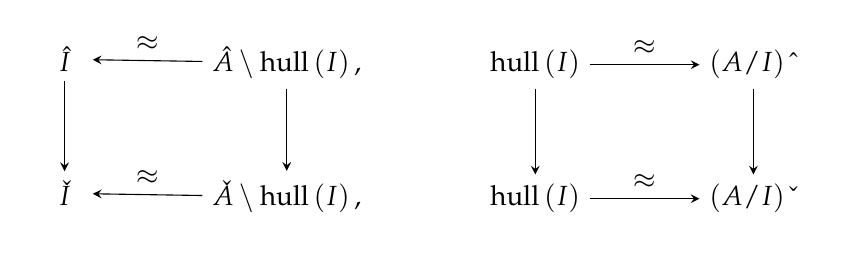
\begin{tikzpicture}
			\matrix (m) [matrix of math nodes,row sep=3em,column sep=4em,minimum width=2em]
			{
				\hat I   & \hat A\setminus \mathrm{hull}\left( I\right),  &\mathrm{hull}\left( I\right) &	\left( A/I\right)\hat~ \\ 
				\check I  &  \check A\setminus \mathrm{hull}\left( I\right), & \mathrm{hull}\left( I\right) & 	\left( A/I\right)\check~\\};
			\path[-stealth]
			(m-1-2) edge node [above] {$\approx $} (m-1-1)
			(m-1-3) edge node [above] {$\approx$} (m-1-4)
			(m-2-2) edge node [above] {$\approx$} (m-2-1)
			(m-2-3) edge node [above] {$\approx$} (m-2-4)
			(m-1-1) edge node [right]  {} (m-2-1)
			(m-1-2) edge node [right]  {} (m-2-2)
			(m-1-3) edge node [right] {} (m-2-3)
			(m-1-4) edge node [right] {} (m-2-4);
		\end{tikzpicture}
		\\ 	
		
	\end{enumerate}
	
\end{theorem}

	If $B\subset A$  is a hereditary $C^*$-subalgebra evenly covered by $\left(C_0\left(\sX \right), \widetilde{A}, G, \lift \right)$ (cf. Definition \ref{evenly_defn}) then there is a connected open subset $\sU \subset \sX$ with $B \cong \sU$. From the Definition \ref{evenly_defn} it follows that $\mathfrak{Gelfand}\left(\lift \right)^{-1}\left(\sU\right)$ is the disjoint union of homeomorphic to $\sU$ connected open subsets of  $\mathfrak{Gelfand}\left(\widetilde A \right)$, i.e. the map $\mathfrak{Gelfand}\left(\lift \right)$ is a covering. If $\widetilde A$ is not commutative then there is $\widetilde x \in \mathfrak{Gelfand}\left(\lift \right)$ with
	$$
\dim \widetilde A / \widetilde x > 1.	
	$$. From the condition (b) of the Definition \ref{fin_pre_defn} it follows that 
	$$
\dim C_0\left( \sX\right) / \mathfrak{Gelfand}\left(\lift \right)\left( \widetilde x\right) > 1.	
	$$
	It is impossible so $\widetilde A\cong C_0\left(\mathfrak{Gelfand}\left(\widetilde A\right) \right)$ is a commutative $C^*$-algebra. Thus there is an 1-1 correspondence between topological and noncommutative coverings of $C_0\left(\sX \right)$. From the Definition \ref{fund_den} that the fundamental group of $C_0\left(\sX \right)$ if it exists is isomorphic to $\pi_1\left( \sX\right)$. 
\subsection{Hausdorff blowing-up}
\subsubsection{Basic construction}

\begin{definition}\label{blowing_defn}
	Any  commutative $C^*$-subalgebra $C\cong C_0\left( \sY\right) \subset M\left(A \right)$ is said to be   \textit{Hausdorff blowing-up} of $A$ if  both sets
	\be\label{blowing_eqn}
	\begin{split}
		C_c\left( \sY\right)A \bydef \left\{fa| f \in C_c\left( \sY\right)\quad a \in A \right\},\\
		AC_c\left( \sY\right) \bydef \left\{af| f \in C_c\left( \sY\right)\quad a \in A \right\}
	\end{split}
	\ee
	are dense in $A$.
\end{definition}

\begin{remark}\label{blowing_rem}
	$C_c\left( \sY\right)A$ is dense in $A$ if and only if $AC_c\left( \sY\right)$ is dense in $A$ (cf. equations \eqref{blowing_eqn}), i.e. both equations ]\eqref{blowing_eqn} are equivalent.
\end{remark}

%\begin{empt}\label{blowing_k_theory_empt}
%	If $A$ be is  stable $C^*$-algebra then $A \cong \K\otimes A\cong A\otimes \K$. Moreover  if  $C_0\left( \sY\right) \subset M\left( A\right)$ be Hausdorff blowing-up then one has a  natural action 
%	\bean
%	C_0\left(\sY \right)\times  \left(A\otimes \K \right)\to A\otimes \K
%	% \left(\K\otimes A\right)\times C_0\left(\sY \right)\to A\otimes \K 
%	\eean 
%	Using it one can one can construct an  injective $*$-homomorphism  !!!
%	$$
%	\left(C_0\left(\sY \right) \otimes \K \right) \to A
%	$$
%	This homomorphism yields homomorphisms of $K$-theory
%	\bea\label{blowing_k0_eqn}
%	K^0\left(\sY \right)\cong K_0\left(C_0\left( \sY\right)  \right) \to K_0\left( A\right),\\\label{blowing_k1_eqn}
%	K^1\left(\sY \right)\cong K_1\left(C_0\left( \sY\right)  \right) \to K_1\left( A\right).
%	\eea 
%	If $A$ is an  irrational rotation algebra of torus then the map $K_1\left(C_0\left( \sY\right)  \right) \to K_1\left( A\right)$ is an isomorphism.
%\end{empt}
%\begin{example}\label{blowing_hausdorff_exm}	If $A$ is a  given by \eqref{cross_mult_eqn} $C^*$-algebra with Hausdorff spectrum $\sX$  then from the Theorems \ref{oa_haus_prim_thm} and  \ref{dauns_hofmann_thm} one has the natural inclusion $C_0\left(\sX \right) \hookto M\left( A\right)$, which is Hausdorff blowing-up.
%\end{example}

\begin{definition}\label{blowing_ideals_au_ua_defn}
	Let  $ C_0\left( \sY\right)\subset  M\left( A\right) $ be  Hausdorff blowing-up of $A$ (cf. Definition \ref{blowing_defn}), and let $\sU \subset \sY$ be an open subset. Both   left and right  closed ideals $A_\sU$  and $_\sU A$ of $A$ generated by sets 	$AC_0\left( \sU\right)$ and $C_0\left( \sU\right)A$ are the \textit{left} $\sU$-\textit{ideal} and the \textit{right} $\sU$-\textit{ideal} respectively. A hereditary $C^*$-subalgebra of $A$
	\be\label{blowing_hereditary_u_eqn} 
	\begin{split}
		_\sU A_\sU \bydef	~	_\sU A\cap  A_\sU = A^*	_\sU \cap  A_\sU\\ %(\text{cf. Definition \ref{hered_defn} and the Lemma \ref{hered_bab_lem}}).
	\end{split}
	\ee	
	is the $ \sU$-\textit{subalgebra}.
	
\end{definition}


\begin{lemma}\label{blowing_compact_lem}
	If $C\cong C_0\left( \sY\right) \subset M\left(A \right)$ is    {Hausdorff blowing-up} of $A$  (cf. Definition \ref{blowing_defn}	for any $a \in A$ and $\eps > 0$ following conditions hold:
	\begin{enumerate}
		\item[(i)] there is a positive $f \in C_c\left( \sY\right)_+$ with 
		\be\label{blowing_compact_eqn}
		\begin{split}
			\left\| f  \right\| \le 1,\\
			\left\| a - af  \right\|< \eps,\\
			\left\| a - fa \right\|< \eps,\\
			\left\| a - faf  \right\|< \eps,
		\end{split}
		\ee
		\item[(ii)] there are an open subset $\sU \subset \sY$ with compact closure and $b \in ~_\sU A_\sU$ such that
		\be\label{blowing_compact_b_eqn}
		\begin{split}
			b \in  ~_\sU A_\sU,\\
			\left\| a - b \right\|< \eps.
		\end{split}
		\ee
	\end{enumerate}
\end{lemma}
\begin{proof}(i)
	If $g \in C_c\left( \sY\right)$ then $g = fg = gf$ for any positive $f \in C_c\left( \sY\right)_+$ such that
	\bean
	\left\| f \right\|= 1,\\
	f\left(\supp g \right) = 1.
	\eean 
	If $f' \in C_c\left( \sY\right)$ and $c' \in A$ such that
	$\left\|a-f'c' \right\| < \eps/4$ (cf. equation \eqref{blowing_eqn}) then there for any positive $f_1$ such that $\left\| f_1 \right\|= 1$, $~f_1\left(\supp f' \right) = 1$ one has
	\bean
	\left\|f_1\left( a-f'c \right) \right\|\le \left\|f_1 \right\|\left\|a-f'c \right\|\le \frac{\eps}{4},\\
	\left\|a-f_1a \right\| < \left\|f_1a - f_1f'c\right\|+ \left\|a - f_1f'c\right\|\le \frac{\eps}{2}
	\eean
	Similarly 	If $f'' \in C_c\left( \sY\right)$ and $c''/ \in A$ such that
	$\left\|a-f'c'' \right\| < \eps/4$ then for any positive for any positive $f_2$ such that $\left\| f_2 \right\|= 1$, $~f_1\left(\supp f' \right) = 1$ one has
	\bean
	\left\|a-a f_2 \right\| <  \frac{\eps}{2}
	\eean
	If $f = \max\left(f_1, f_2 \right)$ then $f\left(\supp f' \cup \supp f'' \right)= \{1\}$ 
	and
	\bean
	\begin{split}
		\left\| f  \right\| \le 1,\\
		\left\| a - af  \right\|< \frac{\eps}{2},\\
		\left\| a - fa \right\|< \frac{\eps}{2},\\
	\end{split}
	\eean
	On the other hand
	\bean
	\left\| a - faf \right\|\le \left\| a - fa \right\|+ \left\| fa - faf \right\|< \frac{\eps}{2}+ 	\left\| f\right\|\left\|a - fa\right\|< \eps.
	\eean
	(ii) The set $\sU \bydef \left\{y \in \sY | f\left(y\right)\neq 0\right\}\subset \sY$ is open and closure of $\sU$ is the compact set $\supp f$. Moreover  $f a f \in ~_\sU A_\sU$ and  $\left\|a - faf\right\|< \eps$.
	
\end{proof}
%\begin{empt}\label{blowing_compact_supp_empt}
%	If $\left\{\sU_\la\right\}_{\la\in\La}$ is a given by the Corollary	\ref{top_connected_union_cor} family of open subsets of $\sY$ with compact closures then $\sY = \cup_{\la \in \La} \sU_\la$. Since the family is directed the union $A_c \bydef \cup_{\la \in \La} \sU_\la$ is a $*$-subalgebra of $A$. From the Lemma \ref{blowing_compact_lem} it follows that $A_c$ is dense in $A$.
%\end{empt}
%\begin{definition}\label{blowing_compact_supp_defn}
%	The given by \ref{blowing_compact_supp_empt} dense $*$-subalgebra $A_c \subset A$ is said to be the \textit{algebra of compactly supported elements}.
%\end{definition}


\begin{empt} 
	
	We leave to the reader a proof of following equations:
	\be\label{blowing_su_eqn}
	\begin{split}
		_\sU A \bydef \left\{ a \in A~ |~ \forall f \in C_0\left( \sY\right)\quad f\left(\sU \right)= \{0\}  \quad \Rightarrow \quad fa = 0\right\} ,\\
		A_\sU \bydef \left\{ a \in A~ |~ \forall f \in C_0\left( \sY\right)\quad  f\left(\sU \right)= \{0\} \quad \Rightarrow \quad af = 0\right\}
	\end{split}
	\ee
	
	
	\bea\label{blowing_sue1_eqn}
	\sU'\cap \sU'' =\emptyset\quad \Rightarrow\quad A_{\sU'}~_{\sU''}A= \{0\}.
	\eea
	
	From \eqref{blowing_su_eqn} it follows that
	\be\label{blowing_su_inc_eqn}
	\sU'\subset \sU'' \quad \Rightarrow\quad _{\sU'}A \subset~  _{\sU'}A ~\text{ AND } ~A_{\sU'}\subset A_{\sU''}~\text{ AND }~  _{\sU'}A _{\sU'}\subset _{\sU''}A _{\sU''}.
	\ee
\end{empt}

\begin{definition}\label{blowing_support_defn}
	If $C_0\left( \sY\right) \subset M\left(A \right)$ is    {Hausdorff blowing-up} of $A$  (cf. Definition \ref{blowing_defn}),  $a \in A$ and
	$
	\sU_a \bydef\bigcap 
	\left\{\left.{\sU} \subset \sX\right| a\in~_\sU A_{\sU} \right\}
	$
	then the  closure $\sV_a$  of $\sU_a$ is said to be the \textit{support} of $a$. We write $\supp a \bydef \sV_a$.
\end{definition}

\begin{lemma}\label{pedersen_eps_lem}
	Let $\eps > 0$, and let 	 $f_\eps: \R \to \R$ be a continuous function given by 
	\begin{equation}\label{f_eps_eqn}
		f_\eps\left( x\right)  \bydef\left\{
		\begin{array}{c l}
			0 &x \le \eps \\
			x - \eps & x > \eps
		\end{array}\right.
	\end{equation}
	If $A$ is a $C^*$-algebra 
	then one has
	\bea\label{k0_ped_e_eqn}
	K\left( A \right)_0 = \left\{f_\eps \left(a\right) \left|~a \in A_+, \quad \eps > 0 \right.\right\},~~~\\
	\label{kp_ped_e_eqn}
	K\left( A \right)_+ = \left\{a \in A_+ \left|a \le \sum_{j = 1}^n f_{\eps_j}\left(  a_j\right) \quad a_j \in  	K\left( A \right)_0\quad \eps_j > 0\quad j=1,...,n\right.\right\}~~
	\eea
	where both $	K\left( A \right)_0$ and 	$K\left( A \right)_+$ are given by equations \eqref{pedersen_k0_eqn} and \eqref{pedersen_k_plus_eqn} respectively
\end{lemma}
\begin{proof}
	If  $a\in A_+$ and $\eps > 0$ then $f_\eps \left(a\right)= \phi_\eps\left(a \right)$ where  $\phi_\eps \in K(]0, \infty [$ is given by 
	\bean
	\phi_\eps\left( x\right)  =\left\{
	\begin{array}{c l}
		0 &x \le \eps \\
		x - \eps &  \eps \le x \le \left\| a\right\|\\
		2	\left\| a\right\| - \eps - x & \left\| a\right\| \le x \le 2\left\| a\right\|-\eps\\
		0 & x \ge 2 \left\| a\right\| -\eps\\
	\end{array}\right.
	\eean
	It follows that $f_\eps\left(a\right)	\in K\left( A \right)_0$. Conversely  if $a \in	K\left( A \right)_0$ then from \eqref{pedersen_k0_eqn} it turns out that there is $b \in A_+$ and $\varphi \in   K(]0, \infty [$ such that $a = \varphi\left(b\right)$. If  $\supp \varphi \subset \left[\eps, c\right]$ and  $\psi \in C_c\left( \R\right)_+$ is given by
	\bean
	\psi\left( x\right)  =\left\{
	\begin{array}{c l}
		0 &x \le 0 \\
		x &0 \le x \le \eps \\
		\varphi\left(x\right) + \eps &\eps \le x \le c \\
		\eps + c - x&  c \le x \le c+ \eps\\
		0 & x \ge c + \eps
	\end{array}\right.
	\eean
	then $ \varphi = f_\eps  \circ\psi$. It follows that $a = f_\eps\left(b' \right)$ where $b' \bydef \psi\left(b\right)$. So the equation \eqref{k0_ped_e_eqn} is proven. The equation \eqref{kp_ped_e_eqn} is a direct consequence of \eqref{k0_ped_e_eqn} and \eqref{pedersen_k_plus_eqn} ones.
	
\end{proof}





\begin{lemma}\label{blowing_pedersen_compact_lem}
	If  $C_0\left( \sY\right)\hookto M\left( A\right)$ is Hausdorff blowing-up and $a\in A$ belongs to the Pedersen's ideal $K\left(A \right)$ (cf. Definition \ref{pedersen_ideal_defn}) then the support of $a$ (cf. Definition \ref{blowing_support_defn}) is compact
\end{lemma}
\begin{proof}
	If $a \in K\left(A\right)_0$ (cf \eqref{pedersen_k0_eqn}) then from the Lemma  \eqref{pedersen_eps_lem} it follows that there is $\eps > 0$ and $b \in A_+$ such that $a = f_\eps \left( b\right)$ where $f_\eps$ is given by \eqref{f_eps_eqn}. On the other hand  there is a positive element !!!!  $c\in  A_+$  such that $\left\|c - b \right\|  < \eps/2$ and $\supp c$ is compact (cf. Definition  \ref{blowing_defn}).
	If $a \le c$ does not hold and $\rho: A \hookto B\left(\H \right)$ is a faithful  nondegenerate representation  then there is $\xi \in \H$ such that
	\bean\label{blowing_ac_eqn}
	\forall \xi \in \H \quad \left( \xi, \rho\left( a \right) \xi\right) > \left( \xi, \rho\left( c \right) \xi\right)
	\eean
	From $\left\|c - b \right\|  < \eps/2$ if follows that
	\be\label{blowing_acc_eqn}
	\forall \xi \in \H  \quad \left\| \xi \right\| = 1\quad \Rightarrow\quad  \left|\left( \xi, \rho\left( b \right) \xi\right)-\left( \xi, \rho\left( c \right) \xi\right) \right| < \eps/2
	\ee
	On the other hand from $a =f_\eps \left( b\right)> 0$ it follows that there is $\xi \in \H$ and $\la \in \R_+$ such that
	\bean
	\left\| \xi \right\| = 1,\\
	\rho\left(a \right) \xi = \la \xi,\\
	\rho\left(b \right)\xi = \left( \la+\eps \right) \xi,\\
	\rho\left(a \right)\xi = \la  \xi,\\
	\left( \xi, \rho\left( b \right) \xi\right) - \left( \xi, \rho\left( a \right) \xi\right)= \eps
	\eean
	and taking into account \eqref{blowing_acc_eqn} one has
	$$
	\left( \xi, \rho\left( c \right) \xi\right)- \left( \xi, \rho\left( a \right) \xi\right)> \frac{\eps}{2}
	$$
	Above condition contradicts with \eqref{blowing_ac_eqn} so $a \le c$.
	If $\supp a \subsetneqq \supp c$ then there is a nonempty  open set  $\sU \subset \supp a\setminus \supp c$. For any $f \in C_0\left(\sU \right)\setminus \{0\}$ one has
	\bean
	faf^* > 0,\\
	fcf^* = 0.
	\eean
	However it is impossible since $a \le c$, so $\supp a \subsetneqq \supp c$ is not true and $\supp a \subset\supp c$. Thus the set $\supp a$ is a closed subset of the compact set $\supp c$ therefore $\supp a$ is compact. Using this fact and the Definition \ref{pedersen_ideal_defn} we conclude that $\supp a$ is compact for any $a \in K\left( A\right)$. 
\end{proof}
\begin{remark}
	The Lemma \ref{blowing_pedersen_compact_lem} can be regarded as a generalization of the equation  \eqref{peder_c0_eqn}.
\end{remark}
\subsubsection{Properties of Gelfand space}
\begin{lemma}\label{top_tietze_ext_lem}\cite{munkres:topology}
If $\sX$ is a Hausdorff,  locally compact space, and $\sY \subset \sX$ is a compact subspace then the restriction map
\bean
C_c\left(\sX \right) \to C\left(\sY \right) ,\\
f \mapsto f|_{\widetilde\sY}
\eean
is surjective.
\end{lemma}

\begin{lemma}\label{good_blowing_lem}
		Any  Hausdorff blowing-up $C_0\left( \sY\right) \hookto M\left(\widetilde A \right)$ (cf. Definition \ref{blowing_defn}) is a good homomorphism (cf. Definition \ref{good_defn}).
\end{lemma}
\begin{proof}
	The map \eqref{lat_mor_eqn} yields a homomorphism of meet-semilattices
	
	\bean
	\mathfrak{Lattice}\left(\widetilde  A\right) \xrightarrow{\mathfrak{Lattice}\left(\varphi\right)}\mathfrak{Lattice}\left( C_0\left( \sX\right) \right)
	\eean
	which is equivalent to the homomorphism
	\be\label{top_lat_eqn}
	\mathfrak{Lattice}\left(\widetilde  A\right) \xrightarrow{\mathfrak{Lattice}\left(\varphi_{\mathrm{top}}\right)}\mathfrak{Lattice}\left(  \sX \right)
	\ee
	Similarly to \eqref{fil_mor_eqn} one has a mapping
	\bean
	\begin{split}
		\mathfrak{Filters}\left(\widetilde  A\right) \xrightarrow{\mathfrak{Filters}\left(\varphi_R \right)}\mathfrak{Filters} \left( \sX\right)
	\end{split}
	\eean
	If $\widetilde{f}\in \mathfrak{Gelfand}\left(\widetilde  A\right)$ then there is a nontrivial element $\widetilde{a}\in K\left( \widetilde a\right)\setminus\{0\}$  such that 
	\bean
	\forall \widetilde I \in \widetilde f \quad \widetilde a \notin \widetilde I.
	\eean
 From the Lemma \ref{blowing_pedersen_compact_lem} it follows that $\supp \widetilde{a}$ is compact. If $f \bydef \mathfrak{Filters}\left(\varphi_R \right)\left( \widetilde f\right)$ then from the Proposition \ref{top_ultra_thm} it follows that there is at least one point $x \in \supp \widetilde{a}$ with $f \le f_x$ where $f_x \in \mathfrak{Gelfand}\left(C_0\left(\sX \right) \right)$ is the corresponding to $x$ ultrafilter. If $f$ is not an ultrafilter then there is  $x' \in \supp \widetilde{a}$ such that $x' \neq x$ and $f \le f_{x'}$. There are closed neighborhoods $\sU'$ and $\sU''$ of  $x'$ and $x''$ with $\sU'\cap \sU'' = \emptyset$. From the Lemma \ref{top_tietze_ext_lem} there is ${b}\in C_0\left( \sX\right)$ with  $b\left(\sU' \right) = \{1\}$ and $b\left(\sU'' \right) = \{0\}$ .
 If $\widetilde{f'} \in \mathfrak{Filters}\left(\widetilde  A\right)$ is generated by
 $$
 \left\{\widetilde I + \widetilde b \widetilde A\left| \widetilde I \in \widetilde f\right.\right\}
 $$ 
 then $\widetilde{f} \le \widetilde{f'}$ and $\widetilde{f}\neq \widetilde{f'}$. So $\widetilde{f}$ is not an ultrafilter. This fact contradicts with the hypothesis of this Lemma. From this contradiction it follow that $f$ is an ultrafilter. This ultrafilter corresponds to $x \in \supp \widetilde a$. It follows that $f_x\in  \mathfrak{Gelfand}\left(C_0\left(\sX \right)  \right)$.

\end{proof}
\subsubsection{Cohomology of sheaves}
\begin{definition}\label{presheaf_defn}\cite{hartshorne:ag}
	Let $\sX$ be a topological space. A \textit{presheaf} $\mathscr F$ of Abelian groups on  $\sX$ consists of the data
	\begin{itemize}
		\item[(a)] for every open subset $\sU \subseteq \sX$, an Abelian group $\mathscr F\left(\sU\right)$, and 
		\item[(b)] for every inclusion $\sV \subseteq \sU$ of open subsets of $\sX$, a morphism of Abelian groups $\rho_{\sU \sV}:\mathscr F\left(\sU\right) \to \mathscr F\left(\sV\right)$,\\
		subject to conditions
		\begin{itemize}
			\item [(0)] $\mathscr F\left(\sV\right)= 0$, where $\emptyset$ is the empty set,
			\item[(1)] $\rho_{\sU \sU}$ is the identity map, and
			\item[(2)] if $\mathcal W \subseteq \sV \subseteq \sU$ are three open sets, then $\rho_{\sU \mathcal W} = \rho_{\sV \mathcal W }\circ \rho_{\sU \sV}$.
		\end{itemize}
	\end{itemize}
\end{definition}

\begin{definition}\label{sheaf_defn}\cite{hartshorne:ag}
	A \textit{presheaf} $\mathscr F$ on  
	a topological space $\sX$ is a \textit{sheaf}  if it satisfies the following supplementary conditions:
	\begin{itemize}
		\item[(3)] If $\sU$ is an open set, if $\left\{\sV_{\a}\right\}$ is an open covering of $\sU$, and if $s \in \mathscr F\left(\sU\right)$ is an element such that $\left.s\right|_{\sV_{\a}}= 0$ for all $\a$, then $s = 0$;
		\item[(4)] If $\sU$ is an open set, if $\left\{\sV_{\a}\right\}$ is an open covering of $\sU$ (i.e. $\sU = \cup\sV_\a$), and we have elements $s_\a$ for each $\a$, with property that for each $\al, \bt, \left.s_\a\right|_{\sV_{\a}\cap \sV_{\bt}}= \left.s_\bt\right|_{\sV_{\a}\cap \sV_{\bt}}$, then there is an element $s \in \mathscr F\left(\sU\right)$ such that $\left.s\right|_{\sV_\a} = s_\a$ for each $\a$.
	\end{itemize}
	(Note condition (3) implies that $s$ is unique.)
\end{definition}
%\begin{definition}
%	A presheaf \ref{top_x_sheaf_defn} satisfying (4) of the Definition \ref{sheaf_defn} is called \textit{conjunctive} (for $\sU$). (cf. \cite{bredon:sheaf})
%\end{definition}
\begin{definition}\label{sheaf_stalk_defn}\cite{hartshorne:ag}%{stalk_defn}
	If $\mathscr F$ is a {presheaf} on $\sX$, and if $x$ is a point of $\sX$ we define the \textit{stalk} or the \textit{germ} $\mathscr F_x$ 
	\textit{of} $\mathscr F$ \textit{at} $x$ to be the direct limit of groups $\mathscr F\left(\sU\right)$ for all open sets $\sU$ containing $x$, via restriction maps $\rho$.
\end{definition}


\begin{definition}\label{sheaf_mor_defn}\cite{hartshorne:ag}
	If $\mathscr F$  and $\mathscr G$ are presheaves on $\sX$, a \textit{morphism} $\varphi:\mathscr F\to\mathscr G$  consists 
	of a morphism of Abelian groups $\varphi_\sU:\mathscr F\left( \sU\right) \to\mathscr F\left( \sU\right)$ for each open set 
	$\sU$, such that whenever $\sV\subset\sU$ is an inclusion, the diagram 
	\newline
	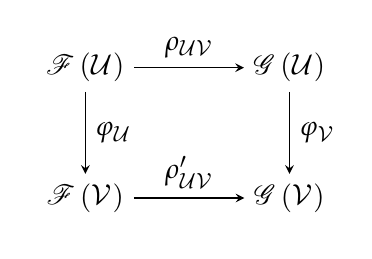
\begin{tikzpicture}
		\matrix (m) [matrix of math nodes,row sep=3em,column sep=4em,minimum width=2em]
		{
			\mathscr F\left( \sU\right)   & \mathscr G\left( \sU\right)\\
			\mathscr F\left( \sV\right)    & \mathscr G\left( \sV\right)\\
		};
		\path[-stealth]
		(m-1-1) edge node [above] {$\rho_{\sU\sV}$} (m-1-2)
		(m-1-1) edge node [right] {$\varphi_\sU$} (m-2-1)
		(m-1-2) edge node [right] {$\varphi_\sV$} (m-2-2)
		(m-2-1) edge node [above] {$\rho'_{\sU\sV}$} (m-2-2);
	\end{tikzpicture}
	\\
	is commutative, where $\rho_{\sU\sV}$ and $\rho'_{\sU\sV}$ are the restriction maps in $\mathscr F$  and $\mathscr G$. If $\mathscr F$  and $\mathscr G$ are sheaves on $\sX$, we use the same definition for a morphism 
	of sheaves. An isomorphism is a morphism  which has a two-sided inverse. 
\end{definition}

\begin{prdf}\label{sheaf_prdf}\cite{hartshorne:ag}
	Given a presheaf $\mathscr F$, there is a sheaf  $\mathscr F^+$ and a morphism $\th: \mathscr F \to \mathscr F^+$, with the property that for any sheaf  $\mathscr G$, and any morphism $\varphi: \mathscr F \to \mathscr G$, there is a unique morphism $\psi:\mathscr F^+\to \mathscr G$ such that $\varphi = \psi \circ \th$. Furthermore the pair $\left(\mathscr F^+, \th\right)$ is unique up to unique isomorphism. $\mathscr F^+$ is called the $\mathrm{sheaf~associated}$ to the presheaf $\mathscr F$. 
\end{prdf}

\begin{empt}\label{sheaf_empt}
	Following text is the citation of the proof of \ref{sheaf_prdf} (cf. \cite{hartshorne:ag}). For any open set $\sU$, let $\mathscr F^+\left(\sU\right)$ be set of functions $s$ from $\sU$ to the union $\bigcup_{x \in \sU}  \mathscr F_x$ of stalks of $\mathscr F$ over points of $\sU$, such that
	\begin{itemize}
		\item [(1)] for each $x \in \sU$, $s\left(x\right)\in \mathscr F_x$, and
		\item[(2)] for each $x \in \sU$, there is a neighbourhood $\sV$ of $x$ contained in $\sU$ and an element $t \in \mathscr F\left(\sV\right)$, such that for all $y \in \sV$ the stalk (germ) $t_y$ of $t$ at $y$ is equal to $s\left(y\right)$.
	\end{itemize}
\end{empt}
\begin{definition}\label{sheaf_inv_im_defn}\cite{hartshorne:ag}
	Let $f: \sX\to \sY$ be a continuous map of topological spaces. For any sheaf  $\mathscr F$ on $\sX$, we define the \textit{direct image} sheaf  $f_*\mathscr F$ on $\sY$ by $\left(f_*\mathscr F\right)\left(\sV\right)= \mathscr F\left(f^{-1}\left(\sV\right)\right)$ for any open set $\sV \subseteq \sY$. For any sheaf  $\mathscr G$ on $\sY$, we define the \textit{inverse image} sheaf  $f^{-1}\mathscr G$ on $\sX$ be the sheaf  associated to the presheaf  $\sU \mapsto \lim_{\sV \supseteq f\left(\sU\right)} \mathscr G\left(\sV\right)$, where $\sU$ is any open set in $\sX$, and the limit is taken over  all open sets $\sV$ of $\sV$ containing $f\left(\sU\right)$.
\end{definition}

\begin{proposition}\label{spectral_sequence_prop}\cite{johnstone:topos}
	%8.17 
	Let $\sX \xrightarrow{f} \sY$ be a continuous map then
	\begin{enumerate}		\item [(i)] 
		if $\mathscr A$ is sheaf of  Abelian group in $\sY$ then we have a homomorphism $H^q\left(\sY, \mathscr A \right) \xrightarrow{} H^q \left(\sX, f^*\mathscr A\right)$ for each $q$ which is functorial in $f$ and natural in $\mathscr A$.
		\item [(ii)] If $\mathscr B$ is a sheaf of Abelian groups in $\sX$ then we have a spectral sequence (Leray spectral sequence) $H^p\left(\mathscr \sY, R^qf_*\left(\mathscr B \right) \right)\Rightarrow H^{p + q}\left(\sX, \mathscr B \right)$ which is natural in $ \mathscr B$.
	\end{enumerate}
\end{proposition}
\begin{remark}
	The above formulation of the Proposition \ref{spectral_sequence_prop} differs from the described in \cite{johnstone:topos} more general one.
\end{remark}
If $C_0\left(\sY \right) \xrightarrow{f} M\left(A \right)$ is Hausdorff blowing-up then 
from the Lemma \ref{good_blowing_lem} it follows that
	\begin{enumerate}		\item [(i)] 
	if $\mathscr A$ is sheaf of  Abelian group in $\sY$ then we have a homomorphism $H^q\left(\sY, \mathscr A \right) \xrightarrow{} H^q \left(\mathfrak{Gelfand}\left(A \right) , f^*\mathscr A\right)$ for each $q$ which is functorial in $f$ and natural in $\mathscr A$.
	\item [(ii)] If $\mathscr B$ is a sheaf of Abelian groups in $\sX$ then we have a spectral sequence (Leray spectral sequence) $H^p\left(\mathfrak{Gelfand}\left( A\right) , R^qf_*\left(\mathscr B \right) \right)\Rightarrow H^{p + q}\left(\sX, \mathscr B \right)$ which is natural in $ \mathscr B$.
\end{enumerate}

\subsubsection{Remarks}
The "blowing-up" word is inspired by following reasons.
\begin{itemize}
	\item Sometimes there is  the natural partially defined  surjective  map from  Hausdorff blowing-up to the spectrum.
	\item  In the algebraic geometry   "blowing-up" means  excluding of singular points  (cf. \cite{hartshorne:ag}).
\end{itemize}


\subsection{Cohomology of continuous trace $C^*$-algebra}


\subsubsection{Gelfand space}
\begin{lemma}\label{hausdorff_spectrum_lem}\cite{rae:ctr_morita}
	Suppose $A$ is a $C^*$-algebra with Hausdorff spectrum $\mathcal{X}$.
	\begin{itemize}
		\item [(a)] If $a, b \in A$ and $\mathfrak{rep}_x\left(a \right)=  \mathfrak{rep}_x\left(b \right)$ for every $x \in  \mathcal{X}$, then $a = b$.
		\item[(b)] For each $a \in A$ the function $x \mapsto \left\|\mathfrak{rep}_x\left(a \right) \right\|$ is continuous on  $\mathcal{X}$, vanishes at infinity and has sup-norm equal to $\left\| a\right\|$. 
	\end{itemize}
\end{lemma}
	\begin{theorem}\label{irred_thm}\cite{pedersen:ca_aut}
	Let $\pi: A \to B\left(\H \right)$ be a nonzero representation of $C^*$-algebra $A$. The following conditions are equivalent:
	\begin{enumerate}
		\item [(i)] there are no non-trivial $A$-subspaces for $\pi$,
		\item[(ii)] the commutant of $\pi\left(A \right)$ is the scalar multipliers of 1,
		\item[(iii)] $\pi\left(A \right)$ is strongly dense in   $B\left(\H \right)$,
		\item[(iv)] for any two vectors $\xi, \eta \in \H$ with $\xi \neq 0$ there is $a \in A$ such that $\pi\left(a \right)\xi = \eta$,
		\item[(v)] each nonzero vector in $\H$ is cyclic for  $\pi\left(A \right)$,
		\item[(vi)]  $A \to B\left(\H \right)$ is spatially equivalent to a cyclic representation associated with a pure state of $A$.
	\end{enumerate} 
\end{theorem}
\begin{definition}\label{abelian_element_defn}\cite{pedersen:ca_aut}
	A positive element in $C^*$ - algebra $A$ is {\it Abelian} if subalgebra $xAx \subset A$ is commutative.
\end{definition}
\begin{definition}\label{type_I_defn}\cite{pedersen:ca_aut}
	We say that a $C^*$-algebra $A$ is \textit{of type} $I$ if each non-zero quotient of $A$ contains a non-zero
	Abelian element. If $A$ is even generated (as $C^*$-algebra) by its Abelian elements we say
	that it is \textit{of type} $I_0$.
\end{definition}
\begin{definition}\label{continuous_trace_c_alt_defn}\cite{rae:ctr_morita}
	%Definition 5.13. 
	A \textit{continuous-trace} $C^*$-\textit{algebra} is a $C^*$-algebra $A$ with Hausdorff
	spectrum $\sX$ such that, for each $x_0\in\sX$ there are a neighbourhood $\sU$ of $x_0$ and $a\in A$ such that $\rep_{ x}\left( a\right) $ is a rank-one projection for all $x \in \sU$.
\end{definition}
If $A$ is a continuous trace $C^*$-algebra  and $I\subsetneqq A$ is a closed  left ideal then from the Lemma \ref{hausdorff_spectrum_lem} it follows that  there are $\eps > 0$,  $~a \in A$ and an irreducible representation $\rho: A \to B\left( \H\right)$ with
\be\label{abelian_ineq_eqn}
\forall a' \in I \quad \left\|\rho\left(a - a' \right)  \right\| > \eps.
\ee
On the other hand $A$ is a $C^*$-algebra of type $I_0$. From this fact one can deduce that there is a satisfying to \eqref{abelian_ineq_eqn}  Abelian element. There is $\xi \in \H$ such that $\rho\left(a \right)= \xi \left\rangle \right\langle \xi$. From (v) of the Theorem \ref{irred_thm} it follows that $\H = \rho\left(A \right) \xi$. If $\xi \in \rho\left(I\right) \xi$ then $a \in I$. It is impossible so $\C\xi \cap \rho\left(I\right) \xi = \{0\}$. There are $\xi^\parallel \in  \rho\left(I\right) \xi$ such that if $\xi^\perp \bydef \xi - \xi^\parallel$ then $\xi^\perp\perp  \rho\left(I\right) \xi$. So for any closed left ideal there is one irreducible representation with $\rho\left( I\right)\xi \neq \H$. The spectrum $\sX$ of $A$ is  Hausdorff. If there are $x', x'' \in \sX$ with $x' \neq x''$ and $ \rho_{x'}\left(I\right)\xi' \neq \H'$, $\rho_{x''}\left(I\right)\xi'' \neq \H''$ then there is $f \in C_0\left( \sX\right)$ such that $f\left(x' \right)  = 0$ and  $f\left(x'' \right)  = 0$. If $I'\bydef I' + Af$ then $I'$ is a closed left ideal such that $I \subsetneqq I' \subsetneqq A$. So if $I$ is a maximal left ideal then there is a single point with $\rho\left(I\right) \xi\neq \H$. If codimension of $\rho\left(I\right) \xi\neq \H$ exceds 1 then there if an Abelian element $a'' \in A$ with
$$
\rho\left(I \right) \xi \subsetneqq \rho\left(I \right) \xi + \rho\left(a'' \right) \xi \subsetneqq \H.
$$
\begin{lemma}\label{ctr_gelfand_lem}
	If $A$ is a continuous trace $C^*$-algebra then any element of  $\mathfrak{Gelfand}\left(A \right) $ is given by a pair $\left(x, \xi \right)$ where
	\begin{enumerate}
		\item[(i)] $x$ is a point of the spectrum $\sX$ of $A$ which corresponds to the irreducible representation $\rep_x: A \to B\left( \H_x\right) $,
		\item[(ii)] $\xi \in \C P\left( \H_x\right)$ where $ \C P\left( \H_x\right)$ is a complex projective space.
	\end{enumerate} 
	
\end{lemma}
\begin{proof}
	There is the natural one-to-one correspondence between codimension one planes of any Hilbert space $\H$ and points of   $ \C P\left( \H\right)$.
\end{proof}
Suppose that $A$ is given by a locally trivial  fibre bundle $\F$ with fibre $\K = \K\left(\H \right)$. There is a subbundle $\E \subset \F$ such that fibers of $\E$ are  rank-one positive operators. It givers a bundle $\C P\left(\E \right)$ with fibre $\C P\left( \H\right)$. From the Lemma \ref{ctr_gelfand_lem}  it turns out that there is the natural set theoretic bijective map $\mathfrak{Gelfand}\left(A \right)\cong  \C P\left(\E \right)$.
If $\C P\left(\E \right)_{\mathfrak{Gelfand}}$ is $\C P\left(\E \right)$ supplied with Gelfand topology then there is a bijective continuous map
\be\label{pe_c_eqn}
\phi_{\E} : \C P\left(\E \right)_{\mathfrak{Classic}}\to \C P\left(\E \right)_{\mathfrak{Gelfand}}
\ee
where $\C P\left(\E \right)_{\mathfrak{Classic}}$ is supplied with the classic topology.
In particular if $\sX = \{x\}$ then $A = \K\left(\H \right)$ and $\mathfrak{Gelfand}\left(\K\left(\H \right) \right)\cong  \C P\left(\H \right)$. The subbase of $\mathfrak{Gelfand}\left(\K\left(\H \right)\right) $ contains all sets $\C P\left(\H \right) \setminus L$ where $L$ is a linear subspace of  $\C P\left(\H \right)$. Similarly to \eqref{pe_c_eqn} there is a continuous map 
$$
\phi_{\H} : \C P\left(\H \right)_{\mathfrak{Classic}}\to \C P\left(\H \right)_{\mathfrak{Gelfand}}
$$
Moreover if $\dim \H = n$ then there is a composition
$$
\C P^n_{\mathfrak{Classic}}\to \C P^n_{\mathfrak{Zariski}}\to \C P^n_{\mathfrak{Gelfand}}
$$
where the subscript $_{\mathfrak{Zariski}}$ means the Zariski topology.
If  $\dim \H = \infty$ and $\left\{L_0, L_1, ...\right\}$ is a set of mutually orthogonal codimension one spaces then
$$
\C P\left( \H\right) = \bigcup_{j=0}^\infty \left( \C P\left(\H \right) \setminus L_j\right) 
$$
Similarly 
$$
\C P^n = \bigcup_{j=0}^{n} \left( \C P^n \setminus L_j\right). 
$$
where $\left\{L_0,  ..., L_n\right\}$ is a set of mutually orthogonal codimension one spaces.
\begin{definition}\label{nerve_defn}\cite{spanier:at}
	Given a topological space $\sX$ and a collection $\mathscr W = \left\{\mathcal W\right\}$ of subsets of $\sX$, the \textit{nerve} of $\mathscr W$ denoted by $K\left( \mathscr W\right)$, is  the simplicial complex whose simplexes are finite nonempty subsets of  $\mathscr W$ with nonempty intersections. Thus the vertices of $K\left( \mathscr W\right)$ are nonempty elements of $\mathscr W$.
\end{definition}
\begin{theorem}\label{top_nerve_thm}\cite{bredon:sheaf}
	%PAGE 193 !!! DOWN !!!
	%4.13. Theorem. 
	Let $\mathscr A$ be a sheaf of Abelian groups  on $\sX$ and let $\mathscr U = \left\{\sU_\a\right\}_{\a \in I}$ an open covering  of $\sX$ having the property that $H^p\left( \sU_{\sigma};\mathscr A \right)= 0$  for $p > 0$ and
	all $\sigma \in K\left(\mathscr U \right)$ in the nerve of covering (cf. Definition \ref{nerve_defn}). Then there is a canonical isomorphism
	\be
	H^*\left(\sX, \mathscr A \right) \cong \check H^*\left( \mathscr U; \mathscr A\right). 
	\ee
\end{theorem}
If $F$ is an Abelian group and $\mathscr F$ is a corresponding constant sheaf on $\C P\left(\H \right)_{\mathfrak{Classic}}$  and $\mathscr W= \left\{ \C P\left(\H \right) \setminus L_j\right\}_{j = 0, 1, ... }$ or  $\mathscr W= \left\{ \C P^n\setminus L_j\right\}_{j = 0,..., n }$ then
\be\label{nerve_eqn}
\begin{split}
\forall \sigma \in K\left(\mathscr W\right)\quad \sU_{\sigma} = \sH \setminus \bigcup_{j = 0}^{n_\sigma} L^\sigma_j,\\
\forall j = 1,..., n \quad L^\sigma_j \text{ is a linear subspace of } \sH \quad \codim_{\R} ~ L^\sigma_j  \ge 2,
\end{split}
\ee
 From the equation \eqref{nerve_eqn} one can deduce if  $K\left(\mathscr W\right)$ is the nerve of $\mathscr W$ (cf. Definition \ref{nerve_defn})  then for each $\sigma \in K\left(\mathscr W\right)$ one has
 \bean H^0\left( \sU^{\mathfrak{Classic}}_{\sigma};\mathscr F_{\mathfrak{Classic}} \right)= F, \\H^p\left( \sU^{\mathfrak{Classic}}_{\sigma};\mathscr F_{\mathfrak{Classic}} \right)= 0
 \eean
 From the Theorem \ref{top_nerve_thm} it turns out that
$$
H^*\left(\C P^n_{\mathfrak{Classic}}, \mathscr F_{\mathfrak{Classic}} \right) \cong \check H^*\left( \mathscr W; \mathscr F_{\mathfrak{Classic}}\right)
$$
Taking into account that $\C P^n \setminus L_j$ is open in $\C P\left(\H \right)_{\mathfrak{Gelfand}}$ for any $j$ one has
$$
H^*\left(\C P\left(\H \right) _{\mathfrak{Classic}}, \mathscr F_{\mathfrak{Classic}} \right) \cong H^*\left(\C P\left(\H \right) _{\mathfrak{Gelfand}}, \mathscr F_{\mathfrak{Gelfand}}\right)
$$
The spectrum of $\K\left(\H \right)$ has the single point but cohomology of $\mathfrak{Gelfand}\left(\K\left(\H \right)  \right)$ are not trivial. 
The topology of $\C P\left(\E \right)_{\mathfrak{Gelfand}}$ is the hybrid of Hausdorff and non Hausdorff topology. The following Lemma is a consequence of the Theorem \ref{top_nerve_thm}.
\begin{lemma}
	Let $F$ is an Abelian group.
	Let $\pi :  \C P\left(\E \right)_{\mathfrak{Classic}}\to \sX$ be the natural surjective mapping 
	If $\sX = \bigcup_{\mathcal W \in \mathscr W}  \mathcal W$ where: 
	\begin{itemize}
		\item for any $\mathcal W \in \mathscr W$ one has $\pi^{-1}\left(\mathcal W \right) \cong \mathcal W\times \C P\left( \sH\right)_{\mathfrak{Classic}}$,
		\item $H^p\left( \sU,\mathscr F_{\mathfrak{Classic}} \right)= {0}$  for all $\sU \in K\left(\mathscr W \right)$ and $p> 0$.
	\end{itemize}	
	then there is the natural isomorphism
	$$
	H^*\left(\mathfrak{Gelfand}\left(A \right),\mathscr F_{\mathfrak{Gelfand}}  \right) \cong H^*\left(\C P\left(\E \right) _{\mathfrak{Classic}}, \mathscr F_{\mathfrak{Classic}} \right) 
	$$ 
	where both $\mathscr F_{\mathfrak{Classic}}$ and $\mathscr F_{\mathfrak{Gelfang}}$ are corresponding to $F$ locally constant sheaves.
\end{lemma}


\subsection{$C^*$-algebras of foliations}
\subsubsection{Groupoids}
	\begin{definition}\label{groupoid_defn}\cite{connes:ncg94}
	% 104
	A \textit{groupoid} consists of a set $\G$, a distinguished subset $\G^0\subset\G$, two maps
	$r, s : \G\to \G^0$ and a law of composition
	$$
	\circ: \G^2\bydef\left\{\left.\left(\ga_1,\ga_2 \right) \in \G\times\G~\right| s\left(\ga_1\right)= r\left(\ga_2\right)\right\}\to \G
	$$
	such that
	\begin{enumerate}
		\item $s\left(\ga_1\circ\ga_2\right)=s\left(\ga_2\right), \quad r\left(\ga_1\circ\ga_2\right)=r\left(\ga_1\right)\quad \forall\left(\ga_1, \ga_2 \right) \in \G$
		\item $s\left(x\right)=r\left(x\right)=x \quad\forall x\in\G^0$
		\item $\ga\circ s\left(\ga\right)= r\left(\ga\right)\circ\ga = \ga\quad \forall\ga\in\G$
		\item $\left( \ga_1\circ\ga_2\right) \circ\ga_3=\ga_1\circ\left( \ga_2\circ\ga_3\right) $
		\item Each $\ga \in\G$ has a two-sided inverse $\ga^{-1}$, with $\ga\circ\ga^{-1}=r\left(\ga\right)$, $\ga^{-1}\circ\ga=r\left(\ga\right)$.
	\end{enumerate}
	The maps $r$, $s$ are called the \textit{range} and \textit{source} maps.
\end{definition}

\begin{definition}
	% Definition 1.11.
	Let $\G$ be a groupoid. A $\G$-\textit{bundle} $(A,L)$ is a $\mathscr C$ - bundle $A$ together
	with a homomorphism $L : G \to \text{Iso} (A)$ such that $L^0: \G^0\to A^0$ is a bijection . (We will often identify $\G^0$ and $A^0$). When  $\mathscr C$  is the category of Abelian groups, one speaks of a
	$\G$-\textit{module bundle}.
\end{definition}
\begin{empt}\label{groupoig_gn_empt}
	Given a $\G$-module bundle $( A , L )$, one can form the following cochain complex. Let
	us first define $\G^n$ for any $n\in\N$. The sets $\H^0$ , $\G^1\bydef \G$ and $\G^2$ have already been defined. For $n> 2$, $\quad \G^n$ is the set of $n$-tuples $(x_0 . . . . . x_{n-1}) \in \G\times...\times \G$ such that for $
	j = 1 , . . . , n - 1$ , $\quad x_j$ is composable with its left  neighbor. A $n$-cochain is a function from $G^n$ to $A$ which satisfies the conditions
	\begin{enumerate}
		\item[(i)] $p\circ f(x_0 . . . . . x_{n-1}) = d(x_0)$ and
		\item[(ii)] if $n > 0$ and for some $j = 0, . . . , n - 1$ , $\quad x_0 \in \G^0$, then $f ( x_0, ..., x_j , ..., x_{n-1})\in A^0$.
	\end{enumerate}
	The set $C^n\left(\G, A\right)$ of $n$-cochains is an Abelian group under point-wise addition. The
	sequence 
	\bean
	0 \to C^0\left( \G, A\right)\to C^0\left( \G, A\right)\to C^1\left( \G, A\right)\to...\to  C^n\left( \G, A\right) \xrightarrow{\delta^n} C^{n + 1}\left( \G, A\right)\to ...
	\eean
	where 
	\be\label{groupoid_b_eqn}
	\begin{split}
		\delta^0f(x)\bydef L(x)\quad  f\circ s(x) - f \circ r ( x ),\\
		\delta^n(f(x_0 ,..., x_n) = L ( x_0 ) f ( x_1,..., x_n) +\\+ \sum_{j=1}^n (-1)^j
		f ( x_0 ,..., x_{j-1}x_j . . . . . x_{n-1})+(-1)^{n-1} f ( x_0 , . . . , x_{n-1}) \quad  n > 0,
	\end{split}
	\ee
	
	is a cochain complex.
\end{empt}	
\begin{definition}\label{groupoid_cocycle_defn}
	The group of $n$-cocycles of this complex will be denoted by $Z^n(\G,A)$,
	the group of $n$-coboundaries will be denoted by $B^n(\G,A)$ and the $n$-th cohomology group
	$Z^n(\G,A)/B^n(\G,A)$ will be denoted by $H^n(\G,A)$.
\end{definition}

\begin{definition}\label{groupoid_topological_defn}\cite{renault:gropoid_ca}
	A \textit{topological groupoid} consists of a groupoid $\G$ and a topology compatible with the groupoid structure:
	\begin{enumerate}
		\item [(a)] $\G \to \G \quad x \mapsto x^{-1}$ is continuous,
		\item [(b)] $\G^2\to \G\quad \left(x,y\right)\mapsto xy$ is continuous where $\G^2$ has the induced topology from $\G \times \G$.
	\end{enumerate}
\end{definition}

\begin{remark}\cite{renault:gropoid_ca}
	One has:
	\begin{itemize}
		\item the map $x \mapsto x^{-1}$ is a homeomorphism,
		\item if $\G$ is Hausdorff then $\G^0$ is closed in $\G$,
		\item if $\G^0$ is Hausdorff then  $\G^2$ is closed in $\G \times \G$, $\G^0$ is both a subspace of $\G$ and a quotient of $\G$ (by the map $r$), the induced and the quotient topology coincide.
	\end{itemize}
\end{remark}
\begin{definition}\label{groupoid_haar_defn}\cite{renault:gropoid_ca}
	Let $\G$ be a locally compact groupoid. A \textit{left  Haar system} for $\G$
	consists of measures $\left\{\left.\la^u \right| u \in \G^0\right\}$ on $\G$ such that
	\begin{enumerate}
		\item [(a)] the support $\supp\la^u$ of the measure $\la^u$ is $\G^u$,
		\item [(b)]  (continuity) for any $f \in C_c\left(\G\right)$, $u \mapsto \la(f)(u) = \int f d\la^u$ is continuous, and
		\item [(c)]  (left invariance) for any $x\in \G$ and any $f \in  C_c(\G )$, $\int  f ( x y ) d\la^{s(x)}(y) =
		\int f(y)d\la^{r(x)}(y)$.
		
	\end{enumerate}
\end{definition}

\section{Groupoid $C^*$-algebras}
\paragraph{}
Let $\G$ be a locally compact Hausdorff groupoid with left  Haar system $\left\{\la^u\right\}$ and let $\sigma$ be a continuous 2-cocycle in $Z^2\left(\G, \T\right)$. For $f ,g \in C_c(\G, \sigma )$, let us define
\be\label{groupoid_*_c_eqn}
\begin{split}
	f * g \left(x\right)\bydef 
	\int f ( x y ) g \left( y^{-1}\right)\sigma\left(xy, y^{-1} \right) d\la^{d(x)}(y),\\
	f^* ( x ) \bydef \overline{f ( x^{ -1})}~\overline{\sigma\left(x, x^{-1} \right)}, 	
\end{split}
\ee	
In particular is $\sigma$ is trivial then one has a $*$-algebra
\be\label{groupoid_*_eqn}
\begin{split}
	f * g \left(x\right)\bydef 
	\int f ( x y ) g \left( y^{-1}\right) d\la^{d(x)}(y),\\
	f^* ( x ) \bydef\overline{f ( x^{ -1})} 	
\end{split}
\ee	
which is a specialization of \eqref{groupoid_*_c_eqn}

\begin{empt} % ??? DEFINE NORM ???
	Let $\G$ be a locally compact groupoid with left  Haar system $\left\{\la^u\right\}$ (cf. Definition \ref{groupoid_haar_defn}).  For $f$ and $g\in C_c\left(\G\right)$, let  us define
	\be\label{groupoid_*__defn}
	\begin{split}
		f * g \left(x\right)\bydef 
		\int  f ( x y ) g \left( y^{-1}\right) d\la^{d(x)}(y),\\
		f^* ( x ) \bydef\overline{f ( x^{ -1})} 	
	\end{split}
	\ee
	It is proven in \cite{renault:gropoid_ca} that the equations yield a $*$-algebra. 
\end{empt}
	\begin{definition}\label{top_ind_lim_defn}\cite{candel:foliII}
	
	Let $\sX$ be a locally compact Hausdorff space, and let $C_c\left(\sX\right)$ denote the	space of continuous, compactly supported functions on $\sX$. The natural	topology on $C_c\left(\sX\right)$ is the \textit{inductive limit topology}, defined as follows. A net	$\left\{f_\a\right\}$ in $C_c\left(\sX\right)$ converges to $f$ if there is a compact set $K\subset\sX$ containing	the supports of all $f_\a$ and $f$, and such that $f_\a$ converges uniformly to $f$ on$K$.
\end{definition}
		\begin{definition}\label{f_topology_defn}\cite{rudin:fa}
		Suppose next that $\sX$ is a set and $\mathscr F$ is a nonempty family of mappings $f: \sX \to \sY_f$, where each $\sY_f$ is a topological space. (In many important cases, $\sY_f$ is the same for all $f \in \mathscr F$.) Let $\tau$ be the collection of all unions of finite intersections of sets $f^{-1}\left(\sV  \right)$ with $f\in \mathscr F$ and $\sV$ open in $\sY_f$. Then $\tau$ is a topology on $\sX$, and it is in fact the weakest topology on $\sX$ that makes every 
		$f\in \mathscr F$ continuous: If $\tau'$ is any other topology with that property, then $\tau\subset\tau'$. This $\tau$ is called the \textit{weak topology on} $\sX$ \textit{induced by} $\mathscr F$, or, more 
		shortly, the $\mathscr F$-\textit{topology of} $\sX$.
	\end{definition}
	
\begin{definition}\label{w_topology_defn}\cite{rudin:fa}
	Suppose $X$ is a topological vector space (with topology $\tau$) whose dual $X^*$ separates points on $X$.   The $X^*$-topology (cf. Definition \ref{f_topology_defn}) of $X$ is called the 
	\textit{weak topology} of $X$.
\end{definition}

\begin{definition}\label{groupoid_representation_defn}\cite{renault:gropoid_ca}
	%1.3. D e f i n i t i o n : 
	A \textit{representation} of $C_c\left(\G, \sigma\right)$ on a Hilbert space $\H$ is a $*$-homomorphism $L : C_c\left(\G, \sigma\right) \to B\left(\H \right)$ which is continuous when $C_c\left(\G, \sigma\right)$ has the inductive limit 
	topology (cf. Definition \ref{top_ind_lim_defn}) and $B\left(\H \right)$  the weak operator topology (cf. Definition \ref{weak_topology_defn}), and is such that the linear  span of
	$$
	L\left(f \right) \xi , \quad f \in C_c\left(\G, \sigma\right), \quad \xi \in \H
	$$
	is dense in $\H$.
\end{definition}
\begin{lemma}\label{groupoid_mult_repr_lem}\cite{renault:gropoid_ca}
	%1.13. Lemma : 
	If $L$ is a representation of $C_c\left(\G, \sigma\right)$, there exists a unique representation
	$M$ of $C_c\left(\G^0\right)$ such that for every $h \in C_c\left(\G^0\right)$ and every $f\in C_c\left(\G, \sigma\right)$, $L\left(h f \right)= M\left(h \right)L\left(f \right)$  and
	$L\left(fh \right)= L\left(f \right)M\left(h \right)$. 
\end{lemma}


\begin{definition}\label{foli_groupoid_red_defn}\cite{renault:gropoid_ca}
	If $\Pi$ is the set of irreducible representations of $\C\left[\G \right]$ then the completion of $\C\left[\G \right]$ with respect to $C^*$-norm
	\be\label{groupoid_red_norm}
	\left\| a\right\|_r = \sup_{\pi\in \Pi}\left\|\pi\left( a\right)\right\| 
	\ee
	is said to be the \textit{reduced algebra} of $\G$. It will be denoted by $C^*_r\left(\G\right)$.
\end{definition}
\begin{empt}\label{groupoid_reg_empt}\cite{renault:gropoid_ca}
	Let $\sigma$ be a 2-cocycle and $\mu$ a quasi-invariant measure. Consider the measurable
	field of Hilbert space $\left\{L^2\left(\G, \la^u \right) \right\}_{u \in \G^0}$ with square integrable sections
	$\int^\oplus L^2\left(\G, \la^u \right) d\mu\left( u\right)= L^2\left(u \right)$. For $x\in \G$, define $L_u\left( x\right)$  mapping $L^2\left( \G, \la^{d\left( x\right) }\right)$  to
	$L^2\left( \G, \la^{r\left( x\right) }\right)$ by $L_u\left( x\right)\xi\left( y\right) \bydef \sigma\left( x, x^{-1}\right) \xi\left( x^{-1}y\right)$. This yields a given by 
	\be\label{groupoid_reg_eqn}
	L_u :  C_c\left(\G, \sigma\right)\to B\left(L^2\left(u \right)  \right) 
	\ee
	$\sigma$-representation of $\G$,
\end{empt}
\begin{definition}\label{groupoid_reg_defn}\cite{renault:gropoid_ca} % 1.8
	The above $\sigma$-representation of $\G$ will be called the $\sigma$-\textit{regular representation
		of $\G$ on $\mu$}. Its integrated form is the \textit{regular representation on $\mu$ of
		$C_c\left(\G, \sigma \right)$}. 
\end{definition}
\begin{proposition}\label{groupoid_reg_prop}\cite{renault:gropoid_ca}%1.11. Proposition :
	$C_c\left(\G, \sigma \right)$ has a faithful family of bounded representations, consisting
	of regular representations.
\end{proposition}
It results from Proposition \ref{groupoid_reg_prop} that the function defined by 
\be\label{groupoid_red_norm_eqn}
\begin{split}
	\left\|\cdot  \right\|_r : C_c\left(\G, \sigma \right)\to \R,\\
	f \mapsto \sup_{u \in \G^0} \left\|L_u\left( f\right)   \right\|,
\end{split}
\ee
where $L_u$ ranges over all representations induced from the unit space, is
a $C^*$ -norm on $ C_c\left(\G, \sigma \right)$ dominated by the $C^*$ -norm $\left\|f  \right\|$.
\begin{definition}\label{groupoid_red_defn}	\cite{renault:gropoid_ca}%2.8. Definition : 
	The \textit{reduced $C^*$ -algebra} $C^*_r\left(\G, \sigma \right)$ of $\G$ is the completion of
	$C^*_r\left(\G, \sigma \right)$ for the reduced norm $\left\|\cdot  \right\|_r$.
\end{definition}
\begin{empt}\label{groupoid_rho_empt}
	If $\G$ is locally compact groupoid with a continuous 2-cocycle in $Z^2\left(\G, \T\right)$ (cf. Definition \ref{groupoid_cocycle_defn}) and a left  Haar system $\left\{\la^u\left| u \in \G^0\right.\right\}$  (cf. Definition \ref{groupoid_haar_defn}) then there is a $*$-algebra $C_c\left(\G, \sigma \right)$ with given by \eqref{groupoid_*_c_eqn} operations.
	If  $\rho: 	C_c\left(\G , \sigma \right)\to B\left(\H \right)$ is a representation in the sense of the Definition \ref{groupoid_representation_defn} then there is a $C^*$-seminorm 
	\be\label{groupoid_semin_eqn}
	\begin{split}
		\left\|\cdot  \right\|_\rho :   	C_c\left(\G , \sigma \right)\to \R,\\
		a \mapsto \left\|\rho\left( a \right)  \right\|
	\end{split}
	\ee
	We suppose that $\rho$ is \textit{faithful}, i.e. $a \neq 0\quad \Rightarrow \quad \rho_c\left(a \right) \neq 0$. The completion of  $C_c\left(\G , \sigma \right)$ with respect to 	$\left\|\cdot  \right\|_\rho$ is a $C^*$-algebra denoted by $C^*_\rho\left(\G , \sigma \right)$
\end{empt}
\begin{definition}\label{groupoid_rho_defn}
	Under the hypotheses \ref{groupoid_rho_empt} we say that the $C^*$-algebra $C^*_\rho\left(\G , \sigma \right)$ is the $\rho$-\textit{completion} of  $C_c\left(\G , \sigma \right)$.
\end{definition}
\begin{remark}\label{groupoid_blowing_rem}
	From the Lemma \ref{groupoid_mult_repr_lem} it follows that there is  natural Hausdorff blowing-up (cf. Definition \ref{blowing_defn})
	\be\label{groupoid_blowing_eqn}
	C_0\left(\G^0 \right)\hookto M\left( C^*_\rho\left(\G , \sigma \right)\right)  
	\ee
\end{remark}
\subsubsection{Foliations and their $C^*$-algebras}
\section{Foliations and pseudogroups}
%\paragraph{}
% Here I follow to \cite{connes:ncg94}
\begin{definition}\cite{connes:ncg94}		
	Let $M$ be a smooth manifold and $TM$ its tangent bundle, so that
	for each $x \in M$, $T_x M$ is the tangent space of $M$ at $x$. A
	smooth subbundle $\mathcal{F}$ of $TM$ is called {\it integrable} if and only if one of
	the following equivalent conditions is satisfied:
	
	\smallskip
	
	\begin{enumerate}
		
		\item[(a)] Every $x \in M$ is contained in a submanifold $W$ of $M$ such that
		$$
		T_y (W) = \mathcal{F}_y \qquad \forall \, y \in W \, ,
		$$
		
		\smallskip
		
		\item[(b)] Every $x \in M$ is in the domain $U \subset M$ of a
		submersion $p : U \to {\mathbb R}^q$ ($q = {\rm codim} \, \mathcal{F}$) with
		$$
		\mathcal{F}_y = {\rm Ker} (p_*)_y \qquad \forall \, y \in U \, ,
		$$
		
		\smallskip
		\item[(c)] $C^{\infty} \left( \mathcal{F}\right)  = \{ X \in C^{\infty} \left(TM\right) \, , \ X_x \in
		\mathcal{F}_x \quad \forall \, x \in M \}$ is a Lie algebra,
		
		\smallskip
		
		\item[(d)] The ideal $J\left( \mathcal{F}\right) $ of smooth exterior differential forms which
		vanish on $\mathcal{F}$ is stable by exterior differentiation.
	\end{enumerate}
	
\end{definition}


\begin{empt}\label{foli_leaf_empt}\cite{connes:ncg94}
	A foliation of $M$ is given by an integrable subbundle $\mathcal{F}$ of $TM$.
	The \textit{leaves} of the foliation $\left(M , \mathcal F\right)$ are the maximal connected
	submanifolds $L$ of $M$ with $T_x (L) = \mathcal{F}_x $, $\forall \, x \in L$,
	and the partition of $M$ in leaves $$M = \cup
	L_{\alpha}\,,\quad\alpha \in X$$ is characterized geometrically by
	its ``local triviality'': every point $x \in M$ has a neighbourhood
	$\mathcal U$ and a system of local coordinates
	$(x^j)_{j = 1 , \ldots , \dim V}$ called
	{\it foliation charts}, so
	that the partition of $\mathcal U$ in connected components of
	leaves corresponds to the partition of 
	\begin{equation*}
		{\mathbb
			R}^{\dim M} = {\mathbb R}^{\dim \mathcal F} \times {\mathbb R}^{\text{codim}
			\, \mathcal F}
	\end{equation*}
	in the parallel affine subspaces 
	$
	{\mathbb R}^{\dim \mathcal F}
	\times {\rm pt}$.
	The corresponding foliation will be denoted by
	\begin{equation}\label{fol_chart_eqn}
		\left(\R^n, \mathcal{F}_p \right) 
	\end{equation}
	where $p = \dim   \mathcal{F}_p$.
	To each foliation $\left(M, \mathcal{F}\right)$ is canonically associated a $C^*$- algebra
	$C^*_r (M, ~\mathcal{F})$ which encodes the topology of the space of leaves.  To
	take this into account one first constructs a manifold $\mathcal G$, $\dim
	\, \mathcal G = \dim \,M + \dim \,\mathcal F$. 
\end{empt}
\begin{definition}\label{foli_trans_defn}\cite{candel:foliI}
	Let $N \subset M$ be a smooth submanifold. We say that $\sF$ is \textit{transverse} to $N$ (and write $\sF\pitchfork N$) if, for each leaf $L$ of $\sF$ and each point $x \in L\cap N$, $T_x\left(L \right)$ ans $T_x\left(N \right)$ together span $T_x\left( M\right)$. At the other extreme At the other extreme, we say that $\sF$ is tangent to $N$ if, for each leaf $L$ of $\sF$, either $L \cap N = \emptyset$ or $L \subset N$.
\end{definition}
The symbol $\mathbb{F}^p$ denotes either the full Euclidean space $\R^p$ or Euclidean half space $\mathbb{H}^p = \left\{\left.\left(x_1,..., x_n \right) \in \mathbb{R}^p\right| x_1 \le 0 \right\}$.
\begin{definition}\label{foli_rect_defn}\cite{candel:foliI}
	A rectangular neighbourhood in $\mathbb{F}^n$ is an open subset of the form $B = J_1\times...\times J_n$, where each $J_j$ is a (possibly unbounded) relatively open interval in the $j^{\text{th}}$ coordinate axis. If $J_1$ is of the form $\left( a,0\right]$, we say that $B$ has boundary $\partial B\left\{\left(0, x_2,..., x_n \right)\right\}\subset B$.	%In the following, we will consider coordinate charts that have values in F" x F", allow !!! ADMIT !!!ing the possibility of manifolds with boundary and (convex) COI'Ile1'S.
\end{definition}
\begin{definition}\label{foli_chart_defn}\cite{candel:foliI}
	% 	Definition 1.1.17 \\
	Let $M$ be an $n$-manifold. A \textit{foliated chart} on $M$ of codimension $q$ is a pair $\left(\sU, \varphi)\right)$, where $\sU\subset M$ is open and $\varphi : \sU \xrightarrow{\approx} B_\tau\times B_\pitchfork$ is a diffeomorphism, $B_\pitchfork$ being a rectangular neighbourhood in $\mathbb{F}^q$ and $B_\tau$ a rectangular neighbourhood in $\mathbb{F}^{n-q}$. The set $P_y = \varphi^{-1}\left(B_\tau \times \left\{y\right\} \right)$ , where $y \in B_\pitchfork$, is called a \textit{plaque} of this foliated chart. For each $x \in B_\tau$, the set  $S_x=\varphi^{-1}\left(\left\{x\right\} \times B_\pitchfork \right)$  is called a \textit{transversal} of the foliated chart. The set $\partial_{\tau}\sU = \varphi^{-1}\left(B_\tau \times \left(\partial B_\pitchfork \right)  \right)$ is called the \textit{tangential boundary} of $\sU$ and $\partial_{\pitchfork}\sU = \varphi^{-1}\left(\partial \left( B_\tau\right)  \times \partial B_\pitchfork \right)$ is called the \textit{transverse boundary} of $\sU$.
\end{definition}

\begin{definition}\label{foliated_manifold_defn}\cite{candel:foliI}
	Let $M$ be an $n$-manifold, possibly with boundary and corners, and let $\sF= \left\{L_\la\right\}_{\la \in \La}$ be a decomposition  of $M$ into connected, topologically immersed submanifolds of dimension $k=n-q$. Suppose that $M$ admits an atlas $\left\{\sU_\a \right\}_{\a \in \mathfrak A}$ of foliated charts of codimension $q$ such that, for each $\a \in \mathscr A$ and each $\la \in \La$, $L_\la \cap \sU_\a$ is a union of plaques. Then $\sF$ is said to be a \textit{foliation} of $M$ of codimension $q$ (and dimension $k$) and $\left\{\sU_\a \right\}_{\a \in \mathscr A}$ l is called a \textit{foliated atlas} associated to $\sF$. Each $L_x$ is called a leaf of the foliation and the pair $\left(M, \sF \right)$  is called a \textit{foliated manifold}. If the foliated atlas is of class $C^r$ ($0 \le r \le \infty$ or $r=\om$), then the foliation $\sF$ and the foliated manifold $\left(M, \sF \right)$. is said to be \textit{of class} $C^r$.
\end{definition}
\begin{definition}\label{fol_res_defn}\cite{candel:foliI}
	If $\left(M,\mathcal F \right)$ is a foliation and $\mathcal{U} \subset M$ be an open subset $\mathcal F|_{\mathcal{U}}$ is the restriction of $\mathcal F$ on ${\mathcal{U}}$ then we say that  $\left(\mathcal{U},\mathcal F|_{\mathcal{U}}\right) $ is the \textit{restriction}   of $\left(M,\mathcal F \right)$ \textit{to}  $\mathcal{U}$. (cf. \cite{connes:ncg94})
\end{definition}
\begin{definition}\label{foli_atlas_defn}\cite{candel:foliI}
	A \textit{foliated atlas} of codimension $q$ and class $C^r$ on the $n$-manifold $M$ is a $C^r$-atlas $\mathfrak{A}\bydef\left\{\sU_\a \right\}_{\a \in \mathscr A}$  of foliated charts of codimension $q$ which are \textit{coherently foliated} in the sense that, whenever $P$ and $Q$ are plaques in distinct charts of $\mathfrak{A}$, then $P\cap Q$ is open both in $P$ and $Q$. 
\end{definition}
\begin{definition}\label{foli_coh_atlas_defn}\cite{candel:foliI}
	Two foliated atlases  and $\mathfrak{A}$ on $\mathfrak{A}'$ of the same codimension and smoothness class $C^r$ are \textit{coherent} ($\mathfrak{A}\approx\mathfrak{A}'$) if $\mathfrak{A}\cup\mathfrak{A}'$ is a foliated $C^*$-atlas.
\end{definition}
\begin{lemma}\label{foli_coh_atlas_eq_lem}\cite{candel:foliI}
	Coherence of foliated atlases is an equivalence relation.
\end{lemma}
\begin{lemma}\label{foli_coh_atlas_ass_lem}
	Let  $\mathfrak{A}$ and $\mathfrak{A}'$ be foliated atlases on $M$ and suppose that $\mathfrak{A}$ is associated to a foliation $\sF$. Then $\mathfrak{A}$ and $\mathfrak{A}'$ are coherent if and only if $\mathfrak{A}'$ is also associated to $\sF$.
\end{lemma}
\begin{definition}\label{foli_reg_atlas_defn}\cite{candel:foliI}
	A foliated atlas $\mathfrak{A}\bydef\left\{\sU_\a \right\}_{\a \in \mathscr A}$ of class $C^r$ is said to be \textit{regular} if
	\begin{enumerate}
		\item [(a)] For each $\al \in \mathscr A$, the closure $\overline{\sU}_\al$ of $\sU_\al$ is a compact subset of a foliated chart  $\left\{\sV_\a \right\}$ and $\varphi_\a = \psi|_{\sU_\a }$.
		\item[(b)] The cover   $\left\{\sU_\a \right\}$ is locally finite.
		\item[(c)] if $\sU_\a$ and $\sU_\bt$ are elements of $\mathfrak{A}$, then the interior of each closed plaque $P \in \overline \sU_\a$ meets at most one plaque in $\overline \sU_\bt$.
	\end{enumerate}
\end{definition}
\begin{lemma}\label{foli_reg_atlas_ref_lem}\cite{candel:foliI}
	Every foliated atlas has a coherent refinement that is regular.
\end{lemma}
\begin{thm}\label{foli_thm}\cite{candel:foliI}
	The correspondence between foliations on $M$ and their associated foliated atlases induces a one-to-one correspondence between the set of foliations on $M$.
\end{thm}

We now have an alternative definition of the term "foliation". 
\begin{defn}\label{foli_alt_defn}\cite{candel:foliI}
	A \textit{foliation} $\sF$ of codimension $q$ and class $C^r$ on $M$ is a coherence class of foliated atlases of codimension $q$ and class $C^r$ on $M$.
\end{defn}
By Zorn's lemma \ref{zorn_thm}, it is obvious that every coherence class of foliated atlases contains a unique maximal foliated atlas. 
\begin{defn}\label{foli_max_defn}\cite{candel:foliI}
	A \textit{foliation of codimension} $q$ and class $C^r$ on $M$ is a maximal foliated $C^r$-atlas of codimension $q$ on $M$.
\end{defn}
\begin{empt}\label{foli_topology_empt}\cite{candel:foliII}
	We construct a topology for $\G = \G\left( M, \F\right)$  as follows.
	Let $\ga \in \G$ be an element with $s\left(\ga\right)= x$ and $r\left(\ga\right)= x$ in the leaf
	$L$. Represent $\ga$ by an immersion $\a \left[0, 1\right]\to L$. Embed $\left[0, 1\right]$ in $\R^{\dim L}$
	as a closed straight line segment $I$ from the point $p_0$ to the point $p_1$ in
	$\R^{\dim L}$. Then, for some $\eps > 0$, $\a$ can be extended to an immersion $f$ of the
	open set $B \bydef  \left\{\left.w \in \R^{\dim L} |\right| \left\|w - I \right\| , \eps \right\}$ so that $f|_{B_\eps\left(p_0 \right) }$, respectively
	$f|_{B_\eps\left(p_1 \right) }$, is a coordinate chart around $x$, respectively $y$, in $L$. % By applying	the Reeb stability argument (cf. [I, Proposition 11.4.8]), 
	There is a space $Z$
	homeomorphic to a transversal through $x$ in $M$ so that $f$ can be extended
	to an immersion $F$ of the trivial foliated space $B \times Z$ into $M$, and so that
	$F|_{B_\eps\left(p_0 \right)}\times Z$, respectively 	$F|_{B_\eps\left(p_1 \right)}\times Z$, is a foliation chart around $x$, respectively
	$y$, in $M$. Let $\a_{x,w}$ denote the straight path from $0$ to $w$ in $B_\eps\left(p_0 \right)$),
	and let $\a_{y,w}$ be the straight path from $p_1$ to $w$ in $B_\eps\left(p_1 \right)$. The collection of
	elements $\ga \in G$ that have a representative of the form
	$$
	t \in I \mapsto  F\left(\a_{x,u} \#\a\#  \a_{x,u}\left( t\right), z  \right) 	\in M
	$$
	for some $u \in B_\eps\left(p_0 \right)$, $v \in B_\eps\left(p_1 \right)$ and $z \in Z$, is a neighbourhood $U\left( \ga\right)$  of $\ga$ in
	$\G$. ($\a\#\b$denotes the path $\a$ followed by the path $\b$.) Note that
	this makes sense because an element of G can be represented by at most one
	such path. This neighbourhood $\sU$ is diffeomorphic to $B_\eps\left(p_0 \right)\times B_\eps\left(p_1 \right)\times Z$
	(as a foliated space with leaves $B_\eps\left(p_0 \right)\times B_\eps\left(p_1 \right)\times {z}$).
\end{empt}


\begin{example}\label{foli_fibration_exm}\cite{candel:foliI}
	Let $M$ be an $n$-manifold, $B$ a manifold of dimension $n-k$, $\partial M = \emptyset = \partial B$, and let  $\pi: M \to B$ be a smooth \textit{fiber bundle}. That is there is a $k$-manifold $F$ and, for each $x \in  B$, an open neighbourhood $\sU$ of $x$ in $B$ and a commutative diagram
	\\
	\begin{tikzcd}
		\pi^{-1}\left(\sU \right) \arrow[r, "\varphi"] \arrow[d, "\pi"] & \sU\times F  \arrow[d, "p"]\\
		\sU\arrow[r, "\Id"]& \sU
	\end{tikzcd}
	\\ 
	with $\varphi$ a diffeomorphism  and $p$ the canonical projection 	onto the first factor. Each subspace $\pi^{-1}\left(x \right)$, $x\in B$, is clearly an embedded $k$-manifold diffeomorphic to $F$. The manifold is the \text{base} of the fiber bundle and $F$ is the \textit{fiber}. The \textit{total space} of the bundle is $M$.
\end{example}

\begin{definition}\label{foli_fibration_comes_defn}\cite{candel:foliI} 
	Under the hypotheses of the Example \ref{foli_fibration_exm} we say that the foliated space $\left(M, \F \right)$  \textit{comes from the fibration} $\pi: M \to B$.
\end{definition}

\begin{empt}\label{foli_graph_empt}\cite{candel:foliII}
	Let  $\Pi\left( M,\sF\right)$ be the space of paths on leaves, that is, maps $\a : [0,1] \to M$ that are continuous with respect to the leaf topology on $M$. For such a path  let $s\left(\a \right) = \a\left( 0\right)$  be its source or initial point and let  $r\left(\a \right) = \a\left( 1\right)$ be its range or terminal point. The space $\Pi\left( M,\sF\right)$ has a partially defined multiplication: the product $\a\cdot \bt$ of two elements $\a$ and $\bt$ is defined if the terminal point of $\bt$ is the initial point of $\a$, and the result is the path $\bt$ followed by the path $\a$. (Note that this is the opposite to the usual composition of paths  $\al\#\bt = \bt \cdot \a$ used in defining the fundamental group of a space.)
\end{empt}
\begin{definition}\label{foli_path_space_defn}\cite{candel:foliI}
	Under the hypotheses of \ref{foli_graph_empt} we say that the topological space $\Pi\left( M,\sF\right)$ is the \textit{space of path on leaves}.
\end{definition}
%	\begin{definition}\label{foli_groupoid_defn}\cite{candel:foliI}
	%Definition 2.3.3.
	%		A groupoid $\G$ on a set $\sX$ is a category with inverses, having $\sX$ as its set of objects. For $y,z \in \sX$ the set of morphisms of $\G$ from $y$ to $z$ is denoted by $\G^z_y$.
	%	\end{definition}
\begin{defn}\label{foli_graph_defn}\cite{candel:foliII}
	%	Definition 1.3.1
	The \textit{graph}, or \textit{holonomy groupoid}, of the foliated space $\left( M,\sF\right)$  is the quotient space of $\Pi\left( M,\sF\right)$ by the equivalence relation that identifies two paths $\a$ and $\bt$ if they have the same initial and terminal points, and the loop $\a \cdot \bt$ has trivial germinal holonomy.
	The graph of $\left( M,\sF\right)$ will be denoted by $\G\left(M, \sF\right)$, or simply by  $\G\left( M\right)$ or by $\G$ when all other variables are understood.
\end{defn}
\begin{remark}\label{foli_graph_rem}
	The {holonomy groupoid} is a locally compact topological  groupoid (cf. Definitions \ref{groupoid_defn} and \ref{groupoid_topological_defn}).
\end{remark}
\begin{remark}
	There is the natural surjective continuous map
	\be\label{foli_cov_map_eqn}
	\Phi : \Pi\left( M,\sF\right)\to \G\left( M,\sF\right)
	\ee
	from the space of path on leaves to the foliation graph.
\end{remark}
\begin{proposition}\label{foli_chart_prop}\cite{candel:foliI}
	%	Proposition 1.3.14. \\
	Let $\mathfrak{A}= \left\{\sU_\iota\right\}$ be a regular foliated atlas of $M$. For each finite sequence of indices $\left\{\a_0 ,...,\a_k\right\}$, the product
	\be	\label{foli_chart_eqn}
	\sV_{   \a} =	 \G\left(\sU_{\iota_0} \right)~...~\G\left(\sU_{\iota_k} \right) \in \G\left(M, \sF\right) \quad \a = \left({\iota_0},...,{\iota_k}\right)
	\ee
	is either empty or a foliated chart for the graph $\G$. The collection of all such finite products is a covering of $\G$ by foliated charts. 
\end{proposition}
\begin{theorem}\label{foli_graph_thm}\cite{candel:foliII}
	The graph $\G$ of $\left( M,\sF\right)$ is a groupoid with unit space $\G_0 = M$, and this algebraic structure is compatible with a foliated structure on $\G$ and $M$. Furthermore, the following properties hold.
	\begin{enumerate}
		\item [(i)] The range and source maps $r, s : \G \to M$ are topological submersions. 
		\item[(ii)] The inclusion of the unit space $M \to\G$ is a smooth map. 
		\item[(iii)] The product map $\G\times_M \G \to G$, given by $\left( \ga_1 , \ga_2\right) \mapsto\ga_1 \cdot \ga_2$, is smooth.
		\item[(iv)]  There is an involution $j: \G \to \G$, given by $j\left( \ga\right) = \ga^{-1}$, which is a diffeomorphism of $\G$, sends each leaf to itself, and exchanges the foliations given by the range. 
	\end{enumerate}
	
\end{theorem}

Above definitions refines the equivalence relation coming from
the partition of $M$ in leaves $M = \cup L_{\alpha}$. 
An element $\gamma$ of $\mathcal G$ is given by two points $x = s(\gamma)$,
$y = r(\gamma)$ of $M$ together with an equivalence class of smooth
paths: $\gamma (t)\in M$, $t \in [0,1]$; $\gamma (0) = x$, $\gamma
(1) = y$, tangent to the bundle $\mathcal{F}$ ( i.e. with $\dot\gamma (t)
\in \mathcal{F}_{\gamma (t)}$, $\forall \, t \in {\mathbb R}$) up to the
following equivalence: $\gamma_1$ and $\gamma_2$ are equivalent if and only if
the {\it my} of the path $\gamma_2 \circ \gamma_1^{-1}$ at the
point $x$ is the {\it identity}. The graph $\mathcal G$ has an obvious
composition law. For $\gamma , \gamma' \in G$, the composition
$\gamma \circ \gamma'$ makes sense if $s(\gamma) = r(\gamma')$. If
the leaf $L$ which contains both $x$ and $y$ has no my, then
the class in $\mathcal G$ of the path $\gamma (t)$ only depends on the pair
$(y,x)$. In general, if one fixes $x = s(\gamma)$, the map from $\mathcal G_x
= \{ \gamma , s(\gamma) = x \}$ to the leaf $L$ through $x$, given
by $\gamma \in \mathcal G_x \mapsto y = r(\gamma)$, is the my covering
of $L$.
Both maps $r$ and $s$ from the manifold $\mathcal G$ to $M$ are smooth
submersions and the map $(r,s)$ to $M \times M$ is an immersion
whose image in $M \times M$ is the (often singular) subset
\begin{equation*}\label{subset}
	\{ (y,x)\in M \times M: \, \text{ $y$ and $x$ are on the same leaf}\}.
\end{equation*}
% We assume, for notational convenience, that the manifold $\mathcal G$ is Hausdorff, but as this fails to be the case in very interesting examples I shall refer to \cite{connes:foli_survey} for the removal of this hypothesis.  
For
$x\in M$ one lets $\Omega_x^{1/2}$ be the one dimensional complex
vector space of maps from the exterior power $\wedge^k \,  \mathcal{F}_x$, $k =
\dim F$, to ${\mathbb C}$ such that
$$
\rho \, (\lambda \, v) = \vert \lambda \vert^{1/2} \, \rho \, (v)
\qquad \forall \, v \in \wedge^k \,  \mathcal{F}_x \, , \quad \forall \,
\lambda \in {\mathbb R} \, .
$$
Then, for $\gamma \in\mathcal G$, one can identify $\Omega_{\gamma}^{1/2}$ with the one
dimensional complex vector space $\Omega_y^{1/2} \otimes
\Omega_x^{1/2}$, where $\gamma : x \to y$. In other words
\be\label{foli_om_g_eqn}
\Omega_{\mathcal G}^{1/2}=\, r^*(\Omega_M^{1/2})\otimes s^*(\Omega_M^{1/2})\,.
\ee

%\begin{empt}\cite{candel:foliI}
%	Page 57.
%The fact that the regular foliated atlas $\mathfrak A$ is locally finite, together with the 2nd countability of $M$, implies that $\mathfrak A$ is at most countably infinite. Thus, the disjoint union 
%\be
%S = \bigsqcup_{\iota \in \I} S_\iota
%\ee	
%is a q-manifold that imbeds as a submanifold $S \hookto M$ is  transverse to $\sF$.
%\end{empt}
%\begin{prdf}\label{foli_preudo_grp_prdf} \cite{candel:foliI}
%	Proposition 2.2.6. I \\
%	Let $\mathfrak{A}$ be a regular foliated atlas of class $C^r$ and let $\ga = \left\{\ga_{\a, \b}\right\}_{\a, \b \in \mathfrak{A}}$ be its my cocycle. Then the set $\Ga_{\mathfrak{A}}$ of my transformations is the $C^r$ pseudogroup on $S$ generated by $\ga$, called the $\mathrm{my~pseudogroup}$ of $\mathfrak{A}$.
%\end{prdf}

\begin{empt}\label{foli_sc_haus_empt}\cite{candel:foliII}
	The  groupoid of a foliated space all leaves of which are simply connected is Hausdorff.
\end{empt}

\begin{exercise}\label{foli_haus_exer}\cite{candel:foliII}
	%: Exercise 1.3.8. 
	Prove or decide the following.
	\begin{enumerate}
		\item The graph of a foliated space all leaves of which are simply connected is Hausdorff.
		\item The graph of a foliated space all leaves of which have trivial holonomy is Hausdorff.
	\end{enumerate}	
	%	 (1) The graph of a foliated space all leaves of which are simply connected is Hausdorff. (2) The graph of a foliated space all leaves of which have trivial holo nomy is Hausdorff. (3) The graph of the Reeb foliation of the three-sphere is not Hausdorff. (4) True or false: The graph of a codimension one foliated three manifold containing a Reeb component is not Hausdorff.
\end{exercise}



%	\begin{definition}\label{foli_graph_defn1}
	%		The  manifold $\mathcal G$ called the \textit{graph} (or \textit{my groupoid})
	%		of the foliation  $\left(M, \mathcal{F}\right)$  Denote by $\mathcal G\left(M, \mathcal{F}\right)$ the graph of  $\left(M, \mathcal{F}\right)$.
	%	\end{definition}
\begin{definition}\label{foli_pseudo_defn}\cite{candel:foliI}.
	%	Definition 2.2.4. I \\
	Let $N$ be a $q$-manifold. A $C^r$ pseudogroup $\Ga$ on $N$ is a collection of $C^r$ diffeomorphisms $h : D(h) \xrightarrow{\approx} R(h)$ between open subsets of $N$ satisfying the following axioms. 
	\begin{enumerate}
		\item  If $g, h \in \Ga$  and $R(h) \subset G(g)$, then $g \circ h \in \Ga$
		\item	 If $h \in \Ga$, then $h^{-1} \in \Ga$. 
		\item $\Id_N \in \Ga$. 
		\item If $h \in \Ga$ and $W \subset  D(h)$ is an open subset, then $\left.h\right|_W \in \Ga$. 
		\item If $h:D(h) \xrightarrow{\approx} R(h)$ is a $C^r$ diffeomorphism between open subsets of $N$ and if, for each $w \in  D(h)$, there is a neighbourhood $W$ of $w\in  D(h)$ such that $\left.h\right|_W \in \Ga$, then $h \in \Ga$. 
	\end{enumerate}
	If $\Ga' \subset \Ga$ is also a pseudogroup, it is called a subpseudogroup of $\Ga$.
\end{definition}

\begin{remark}\cite{candel:foliI}
	Any pseudogroup is a groupoid (cf. Definition \ref{groupoid_defn}).
\end{remark}
\begin{remark}\cite{candel:foliI}\label{foli_pseudo_rem}
	In the case of general foliations, the total my group of a foliated bun dle must be replaced by a local analogue called the \textit{my pseudogroup}.
\end{remark}
\begin{remark}\label{foli_groupoid_n_red_defn}\cite{candel:foliI}
	If $\left(M, \sF\right)$ is a foliated manifold and $N$ is a tranversal then
	\be\label{foli_gnn_eqn}
	\G^N_N \bydef \left\{\left. \ga \in \G\left(M, \sF\right)\right| s\left(\ga\right), r\left(\ga\right)\in N\right\}
	\ee
	is	a pseudogroup. 
	
	
\end{remark}
\begin{definition}\cite{candel:foliI}
	In the above situation we say that $\G^N_N$ is a \textit{reduced groupoid}.
\end{definition}

\section{Operator algebras of foliations}\label{foli_alg_subsec}
\paragraph*{}
Here I follow to \cite{candel:foliII,connes:ncg94}.  Since the bundle $\Om^{1/2}$ is trivial (because $\G\left(M, \sF\right)$ admits partitions of unity), a choice of an everywhere positive density $\nu$ allow !!! ADMIT !!!s us to identify $\Ga_c\left(\G\left(M, \sF\right),\Om^{1/2}  \right)$  with $\Coo_c\left( \G\left(M, \sF\right)\right)$. 
The definition of foliated space makes sense even when the underlying topological space fails to satisfy the Hausdorff separation axiom. Non-Hausdorff spaces appear naturally in the theory of foliations. In a graph of a foliated space is not necessary Hausdorff. It will be necessary to use functions with compact support on such spaces. However, a non-Hausdorff space may not have sufficiently many such functions, the basic reason being that compact subsets of a Hausdorff space are not necessarily closed. The non-Hausdorff spaces that will appear here have a particularly simple local structure, and even when it is possible to construct appropriate functions using this local structure, the standard operation of  extension by 0  of local objects to the full space does not pro duce continuous functions. M. Crainic and I. Moerdijk \cite{cra_moe:nhaus} proposed a very natural way of dealing with this problem, and this preliminary section describes it. (That paper develops an extended sheaf  theory for non-Hausdorff manifolds (cf. Appendix \ref{sheaves_nh_sec})).
Here $\sX$ will denote a separable topological space having the structure of a foliated space, but it is not required that the topology be Hausdorff. It is only required that $\sX$ can be covered by countably many open sets homeomorphic to a product $\D \times \mathcal Z$, where $D$ is an open ball in Euclidean $n$-space and $\mathcal Z$ is a separable locally compact Hausdorff space. Let $\mathcal C^\infty$ denote the structure sheaf  of the foliated space $\sX$, that is, the sheaf  of smooth functions on $\sX$. Let $\A$ be a sheaf of $\mathcal C^\infty$-modules over   $\sX$, for instance, the sheaf  of differential forms or other sheaves of smooth sections of foliated vector bundles. For such a sheaf  $\A$ over  $\sX$, let $\A$ denote its Godement resolution: $A'\left(\sU\right)$ is the set of all sections (continuous or not) of $\A$ over $\sU\subset\sX$. For a Hausdorff open subset $\mathcal W$ of $\sX$, let $\Ga_c\left( \mathcal W, \A\right) $ denote the set of continuous compactly supported sections of $\A$ over $\mathcal W$. If $\mathcal W\subset\sU$, then  extension by 0  induces a well defined homomorphism $\Ga_c\left( \mathcal W, \A\right)\to \A'\left(\sU \right)$. For an open subset $\sU$ of $\sX$, let $\Ga_c\left( \mathcal U, \A\right)$ denote the image of the homomorphism $\oplus \Ga_c\left( \mathcal W, \A\right)\to \A'\left(\sU\right)$ (cf. Definition \ref{nh_csoft_gc_defn}). From the equation \eqref{sheaf_inc_eqn} it follows that there is the inclusion
\be\label{foli_incc_eqn}
\Ga_c\left(\mathcal W, \A \right) \hookto \Ga_c\left(\mathcal U, \A \right).
\ee
Let $\G\bydef \G\left(M, \sF \right)$ be a foliation chart. 	The bundle $\Omega_M^{1/2}$ is trivial on $M$, and we
could choose once and for all  a trivialization $\nu$ turning
elements of $\Ga_c \left(\mathcal G , \Omega_{\mathcal G}^{1/2}\right)$ into functions.
Let us
however stress that the usage of half densities makes all the
construction completely canonical.
For $f,g \in \Ga_c \left(\mathcal G , \Omega_{\mathcal G}^{1/2}\right)$, the convolution
product $f * g$ is defined by the equality
\be\label{foli_prod_eqn}
(f * g) (\gamma) = \int_{\gamma_1 \circ \gamma_2 = \gamma}
f(\gamma_1) \, g(\gamma_2) \, .
\ee
This makes sense because, for fixed $\gamma : x \to y$ and fixing $v_x
\in \wedge^k \,  \mathcal{F}_x$ and $v_y \in \wedge^k \,  \mathcal{F}_y$, the product
$f(\gamma_1) \, g(\gamma_1^{-1} \gamma)$ defines a $1$-density on
$G^y = \{ \gamma_1 \in G , \, r (\gamma_1) = y \}$, which is smooth
with compact support (it vanishes if $\gamma_1 \notin\supp f$),
and hence can be integrated over $G^y$ to give a scalar, namely $(f * g)
(\gamma)$ evaluated on $v_x , v_y$.
The $*$ operation is defined by $f^* (\gamma) =
\overline{f(\gamma^{-1})}$,  i.e. if $\gamma : x \to y$ and
$v_x \in \wedge^k \, \mathcal{F}_x$, $v_y \in \wedge^k \, \mathcal{F}_y$ then $f^*
(\gamma)$ evaluated on $v_x , v_y$ is equal to
$\overline{f(\gamma^{-1})}$ evaluated on $v_y , v_x$. We thus get a
$*$-algebra $\Ga_c \left(\mathcal G , \Omega_{\mathcal G}^{1/2}\right)$. 
where $\xi$ is a square integrable half density on $\mathcal G_x$. 
For each leaf $L$ of
$\left(M, \mathcal{F}\right)$ one has a natural representation of this $*$-algebra on the
$L^2$ space of the my covering $\tilde L$ of $L$. Fixing a
base point $x \in L$, one identifies $\tilde L$ with $\mathcal G_x = \{
\gamma , s(\gamma) = x \}$ and defines
\begin{equation}\label{foli_repr_eqn}
	(\rho_x (f) \, \xi) \, (\gamma) = \int_{\gamma_1 \circ \gamma_2 =
		\gamma} f(\gamma_1) \, \xi (\gamma_2) \qquad \forall \, \xi \in L^2
	(\mathcal G_x),\
\end{equation}


Given
$\gamma : x \to y$ one has a natural isometry of $L^2 (\mathcal G_x)$ on $L^2
(G_y)$ which transforms the representation $\rho_x$ in $\rho_y$.
\begin{lemma}\cite{candel:foliII} 
	%	Lemma 1.4.1. \\
	If $f_1 \in \Ga_c\left(\sU_{   \a_1},\Om^{1/2} \right)$ and $f_2 \in \Ga_c\left(\sU_{   \a_2},\Om^{1/2} \right)$ then their convolution is a well-defined element $f_1*f_2 \in \Ga_c\left(\sU_{   \a_1}\cdot\sU_{   \a_2},\Om^{1/2} \right)$
\end{lemma}
%page 24.
%Let $\Ga_c\left( \G,\Om^{1/2}\right)$  be the space of compactly supported smooth sections of $\Om^{1/2}$ over $\G$; its elements are the compactly supported half-densities on G. When G is not Hausdorff, the meaning of c (G,D1/2) is that which was described in Section 1.2. This space will now be given the structure of an algebra with involution. This structure is first described when G is Hausdorff, and the details will then be given when G is arbitrary.

\begin{proposition}\label{foli_repr_prop}\cite{candel:foliII} 
	%Proposition 1.4.5. \\
	If $\sV \subset \G$ is a foliated chart for the graph of $\left(M, \sF\right)$ and $f \in \Ga_c\left(\sV, \Om^{1/2}\right)$ , then $\rho_x\left( f\right)$, given by \eqref{foli_repr_eqn}, is a bounded integral operator on $L^2\left(\G_x \right)$.
\end{proposition}
\begin{empt}\cite{candel:foliII} 
	The space of compactly supported half-densities on $\G$ is taken as given by the exact sequence 
	\be\label{foli_ga_p_eqn}
	\bigoplus_{\a_0\a_1}\Ga_c\left(\sU_{   \a_0\a_1}, \Om^{1/2} \right) \to \bigoplus_{\a_0}\Ga_c\left(\sU_{   \a_0},\Om^{1/2} \right) \xrightarrow{\Ga_\oplus}  \Ga_c\left(\G,\Om^{1/2}\right) 
	\ee
	associated to a regular cover   for $\left((M, \sF)\right)$ as above. The first step for defining a convolution is to do it at the level of $\bigoplus_{\a_0}\Ga_c\left(\sU_{   \a_0}\Om^{1/2} \right)$, as the following lemma indicates. 
\end{empt}




\begin{defn}\label{foli_red_defn}\cite{candel:foliII} 
	% 	Definition 1.4.7.\\
	The \textit{reduced} $C^*$-algebra of the foliated space $\left(M,\sF\right)$ is the completion of $\Ga_c\left( \G,\Om^{1/2}\right)$ with respect to the pseudonorm \be\label{foli_pseudo_norm_eqn}
	\left\|f \right\| =\sup_{x \in M}\left\|  \rho_x\left(f\right)\right\|
	\ee where $\rho_x$ is given by  \eqref{foli_repr_eqn}.
	This $C^*$-algebra is denoted by $C^*_r\left(M,\sF\right)$.
\end{defn} 
An obvious consequence of the construction of 
$C^*_r\left(M,\sF\right)$ is the following. 

\begin{cor}\label{foli_cov_alg_cor}\cite{candel:foliII} 
	%	Corollary 1.4.8.
	Let $M$ be a foliated space and let $\mathfrak{A}$ be a regular cover   by foliated charts. Then the algebra generated by the convolution algebras $\Ga_c\left( \G\left(\sU \right), \Om^{1/2}\right)$, $~\sU\in\mathfrak{A}$ is dense in  $C^*_r\left(M,\sF\right)$.
\end{cor}
\begin{definition}\label{foli_full_defn}\cite{candel:foliII}
	%Definition 1.4.12. 
	The \textit{full} $C^*$-algebra of the foliated space $(M,\F)$, denoted
	by $C^*(M,\F)$, is the completion of $\Ga_c\left(\G,\Om^{1/2}\right)$ with respect to the
	pseudonorm
	\be\label{groupoid_full_norm_eqn}
	\left\|f \right\|_f =\sup_{\pi}\left\|  \rho_x\left(f\right)\right\|
	\ee
	where $\pi$ runs through all the involutive representations of $\Ga_c\left(\G,\Om^{1/2}\right)$ on a
	separable Hilbert space whose restrictions to the graph $\G\left( \sU\right)$  of each foliated
	chart $\sU$ for $(M,\F)$ are weakly continuous for the inductive limit topology
	on $\Ga_c\left(\G,\Om^{1/2}\right)$.	
\end{definition}
\begin{empt}\label{foli_res_inc_empt}\cite{candel:foliII} 
	%	page 29-30.
	Let $\left(M,\sF\right)$ be an arbitrary foliated space and let $\sU\subset  M$ be an open subset.  Then $\left(\sU,\sF|_\sU\right)$ is a foliated space and the inclusion  $\sU\hookto  M$ induces a homomorphism of groupoids $\G\left(\sU \right)\hookto \G$ , hence a mapping
	\be\label{foli_inc_gc_eqn}
	j_\sU : \Ga_c\left(  \G\left(\sU \right) ,\Om^{1/2}\right)  \hookto \Ga_c\left( \G\left( M\right) ,\Om^{1/2}\right)
	\ee
	that is an injective homomorphism of involutive algebras. 
	%	It is proven in \cite{candel:foliII,connes:foli_survey} that any restriction of foliation induces an injective $*$-homomorphism 
	%	\begin{equation}\label{fol_res_hom_eqn}
		%	C^*_r\left(\mathcal{U},\mathcal F|_{\mathcal{U}} \right)\hookto C^*_r\left(M,\mathcal F \right).
		%	\end{equation}
\end{empt}
\begin{prop}\label{foli_res_inc_prop} \cite{candel:foliII} 
	%	Proposition 1.5.5. 
	Let $\sU$ be an open subset of the foliated space $M$. Then the inclusion $\sU \hookto M$ induces an isometry of $C^*_r\left(\sU,\sF|_\sU\right)$  into $C^*_r\left(M,\sF\right)$.
\end{prop}
\begin{lemma}\label{foli_leaf_lem}\cite{candel:foliII} 
	%Lemma 1.4.9. 
	Each element $\ga \in \G$ induces a unitary operator $\rho_\ga : L^2\left(s\left( \ga\right)\right)   \xrightarrow{\approx}  L^2\left(r\left( \ga\right)\right) $   that conjugates the operators $\rho_{s\left(\ga \right)} \left(f \right) $ and $\rho_{r\left(\ga \right)} \left(f \right)$. In particular, the norm of $\rho_x\left(f \right)$  is independent of the point in the leaf through $x$.
\end{lemma}

\begin{lem}\label{foli_point_lem}\cite{candel:foliII} 
	%Lemma 1.4.10. 
	If $f \in \Ga^\infty_c\left(\G, \Om^{1/2}\right)$ does not evaluate to zero at each $\ga \in \G$, then there exists a point $x$ in $M$ such that $\rho_x\left( f\right)  \neq  0$.
\end{lem}
%\begin{defn} \label{foli_full_defn} NECESSARY
%  Definition 1.4.12. The full $C^*$-algebra of the foliated space $\left(M, \sF\right)$ denoted by $C^*_r\left(M, \sF\right)$, is the completion of %c(G,D1/2) with respect to the pseudonorm f=f= sup (f), where runs through all the involutive representations of c (G,D1/2) on a separable Hilbert space whose restrictions to the graph G(U) of each foliated chart U for (M,F) are weakly continuous for the inductive limit ... Because each Rx, x  M, is an involutive representation of the convolution 
%\end{defn}
\begin{definition}\label{foli_fibration_defn}\cite{candel:foliI}
	A foliated space $\left(M, \sF\right)$ is a \textit{fibration} if for any $x$ there is an open transversal $N$ such that $x\in N$ and for every  leaf $L$ of $\left(M, \sF\right)$ the intersection $L\cap  N$ contains no more then one point.
\end{definition}
\begin{prop}\label{foli_one_leaf_prop}
	% Proposition 1.5.1. 
	The reduced $C^*$-algebra of a foliated space $M$ consisting of exactly one leaf is the algebra $\K\left( L^2\left(M \right) \right)$  of compact operators on $L^2\left(M \right)$.
\end{prop}


\begin{prop}\label{foli_tens_comp_prop}\cite{candel:foliII}
	% Proposition 1.5.4. \\
	The reduced  $C^*$-algebra $C^*_r\left(\mathcal N\times \mathcal Z \right)$ of the trivial foliated space $\mathcal N \times \mathcal Z$ is the tensor product $\K\otimes C_0\left(\mathcal Z\right)$, where $\K$ is the algebra of compact operators on $L^2\left(\mathcal N \right)$  and $ C_0\left(\mathcal Z\right)$ is the space of continuous functions on $\mathcal Z$ that vanish at infinity.
\end{prop}
\begin{corollary}\label{foli_tens_comp_cor}\cite{candel:foliII}
	%Corollary 1.5.10. 
	The full $C^*$-algebra of a trivial foliated space $\mathcal N \times \sZ$ is
	the tensor product $\K\left( L^2\left( \mathcal N\right) \right) \otimes C_0\left( \sZ\right)$. 	
\end{corollary}
\subsubsection{Gelfand space}

\section*{Acknowledgment}


\paragraph*{}
 Author would like to acknowledge members of the Moscow State University Seminars
"Noncommutative geometry and topology", "Algebras in analysis" leaded by professors A. S. Mishchenko and  A. Ya. Helemskii for a discussion
of this work. 


\begin{thebibliography}{10}
		\bibitem{arveson:c_alg_invt} W. Arveson. {\it An Invitation to $C^*$-Algebras}, Springer-Verlag. ISBN 0-387-90176-0, 1981.
		
\bibitem{blackadar:ko} B. Blackadar. {\it K-theory for Operator Algebras}, Second edition. Cambridge University Press. 1998.
	
		\bibitem{bredon:sheaf} Bredon, Glen E. (1997), \textit{Sheaf theory}. Graduate Texts in Mathematics, 170 (2nd ed.), Berlin, New York: Springer-Verlag.  ISBN 978-0-387-94905-5, MR 1481706 (oriented towards conventional topological applications), 1997.
\bibitem{bourbaki_sp:gt} N. Bourbaki, {\it Elements of Mathematics. General Topology}, Part 1. \newline HERMANN, \'{E}DITEURS DES SCIENCES ET DAS ARTS \newline 115 Boulevard Saint-Germain. Paris \newline ADDISON-WESLEY PUBLISHING COMPANY. \newline Reading, Massachusets - Palo Ito - London - Don Mills, Ontario \newline A translation of \newline \'{E}L\'{E}MENTS DE MATH\'{E}MATIQUE, TOPOLOGIE G\'{E}N\'{E}RALE, \newline originally published in French by Hermann, Paris. 1966.

\bibitem{candel:foliI}Alberto Candel, Lawrence Conlon. \textit{Foliations I}. Graduate Studies in Mathematics, American Mathematical Society (1999), 1999.


\bibitem{candel:foliII}Alberto Candel, Lawrence Conlon. \textit{Foliations II}. American Mathematical Society; 1 edition (April 1 2003), 2003.


	
\bibitem{connes:ncg94} Alain Connes. {\it Noncommutative Geometry}, Academic Press, San Diego, CA,  661 p., ISBN 0-12-185860-X, 1994.

	\bibitem{hartshorne:ag} Robin Hartshorne. {\it Algebraic Geometry.} Graduate Texts in Mathematics, Volume 52, 1977.
	
	 	
	\bibitem{johnstone:stone_spaces} Peter Johnstone. \textit{Stone Spaces} Cambridge Studies in Advanced Mathematics 3, Cambridge University Press (1982, 1986).
	
	\bibitem{johnstone:topos}Peter Johnstone. \textit{Topos Theory}, L. M. S. Monographs no. 10, Academic Press 1977.
		
			\bibitem{matro:hcm} Manuilov V.M., Troitsky E.V. \textit{Hilbert $C^*$-modules}. % Publication Year: 2005. ISBN-10: 0-8218-3810-5 ISBN-13: 978-0-8218-3810-5 
	Translations of Mathematical Monographs, vol. 226, 2005.
	
\bibitem{munkres:topology} James R. Munkres. {\it Topology.} Prentice Hall, Incorporated, 2000.

	
	\bibitem{murphy}G.J. Murphy. {\it $C^*$-Algebras and Operator Theory.} Academic Press 1990.	
		\bibitem{pedersen:ca_aut}Gert K Pedersen. {\it $C^*$-algebras and their automorphism groups}. London ; New York : Academic Press, 1979.

\bibitem{pedersen:mea_c} Gert K Pedersen.  \textit{Measure Theory for $C^*$-Algebras}. Mathematica Scandinavica (1966) Volume: 19, page 131-145
ISSN: 0025-5521; 1903-1807/e, 1966.
	
	
	\bibitem{rae:ctr_morita} Iain Raeburn, Dana P. Williams. \textit{Morita Equivalence and Continuous-trace $C^*$-algebras}. American Mathematical Soc., 1998.


\bibitem{renault:gropoid_ca} Jean Renault, \emph{A groupoid approach to {$C\sp{\ast} $}-algebras}, Lecture Notes in Mathematics, vol. 793, Springer, Berlin, 1980. 
\bibitem{rudin:fa}Walter Rudin. \textit{Functional Analysis}, Second Edition, McGraw-Hill, Inc. New York St. Louis San Francisco Auckland Bogota Caracas Hamburg Lisbon London Madrid Mexico Milan Montreal New Delhi Paris San Juan Sao Paulo Singapore Sydney Tokyo Toronto, 1991.



	
		\bibitem{spanier:at}
E.H. Spanier. {\it Algebraic Topology.} McGraw-Hill. New York. 1966.

		\bibitem{thomsem:ho_type_uhf} Klaus Thomsen. {\it The homotopy type of the group of automorphisms of a $UHF$-algebra}. Journal of Functional Analysis. Volume 72, Issue 1, May 1987.

\end{thebibliography}



	\end{document}
